% source-sha256: ba814f9e233a6ebd4d3a6b4b9a3e2584aeb23a83a872c9029ab97b60bd8b8d52
% Options for packages loaded elsewhere
\PassOptionsToPackage{unicode}{hyperref}
\PassOptionsToPackage{hyphens}{url}
\documentclass[
]{article}
\usepackage{xcolor}
\usepackage[letterpaper,margin=1in]{geometry}
\usepackage{amsmath,amssymb}
\setcounter{secnumdepth}{-\maxdimen} % remove section numbering
\usepackage{iftex}
\ifPDFTeX
  \usepackage[T1]{fontenc}
  \usepackage[utf8]{inputenc}
  \usepackage{textcomp} % provide euro and other symbols
\else % if luatex or xetex
  \usepackage{unicode-math} % this also loads fontspec
  \defaultfontfeatures{Scale=MatchLowercase}
  \defaultfontfeatures[\rmfamily]{Ligatures=TeX,Scale=1}
\fi
\usepackage{lmodern}
\ifPDFTeX\else
  % xetex/luatex font selection
\fi
% Use upquote if available, for straight quotes in verbatim environments
\IfFileExists{upquote.sty}{\usepackage{upquote}}{}
\IfFileExists{microtype.sty}{% use microtype if available
  \usepackage[]{microtype}
  \UseMicrotypeSet[protrusion]{basicmath} % disable protrusion for tt fonts
}{}
\makeatletter
\@ifundefined{KOMAClassName}{% if non-KOMA class
  \IfFileExists{parskip.sty}{%
    \usepackage{parskip}
  }{% else
    \setlength{\parindent}{0pt}
    \setlength{\parskip}{6pt plus 2pt minus 1pt}}
}{% if KOMA class
  \KOMAoptions{parskip=half}}
\makeatother
\usepackage{color}
\usepackage{fancyvrb}
\newcommand{\VerbBar}{|}
\newcommand{\VERB}{\Verb[commandchars=\\\{\}]}
\DefineVerbatimEnvironment{Highlighting}{Verbatim}{commandchars=\\\{\}}
% Add ',fontsize=\small' for more characters per line
\newenvironment{Shaded}{}{}
\newcommand{\AlertTok}[1]{\textcolor[rgb]{1.00,0.00,0.00}{\textbf{#1}}}
\newcommand{\AnnotationTok}[1]{\textcolor[rgb]{0.38,0.63,0.69}{\textbf{\textit{#1}}}}
\newcommand{\AttributeTok}[1]{\textcolor[rgb]{0.49,0.56,0.16}{#1}}
\newcommand{\BaseNTok}[1]{\textcolor[rgb]{0.25,0.63,0.44}{#1}}
\newcommand{\BuiltInTok}[1]{\textcolor[rgb]{0.00,0.50,0.00}{#1}}
\newcommand{\CharTok}[1]{\textcolor[rgb]{0.25,0.44,0.63}{#1}}
\newcommand{\CommentTok}[1]{\textcolor[rgb]{0.38,0.63,0.69}{\textit{#1}}}
\newcommand{\CommentVarTok}[1]{\textcolor[rgb]{0.38,0.63,0.69}{\textbf{\textit{#1}}}}
\newcommand{\ConstantTok}[1]{\textcolor[rgb]{0.53,0.00,0.00}{#1}}
\newcommand{\ControlFlowTok}[1]{\textcolor[rgb]{0.00,0.44,0.13}{\textbf{#1}}}
\newcommand{\DataTypeTok}[1]{\textcolor[rgb]{0.56,0.13,0.00}{#1}}
\newcommand{\DecValTok}[1]{\textcolor[rgb]{0.25,0.63,0.44}{#1}}
\newcommand{\DocumentationTok}[1]{\textcolor[rgb]{0.73,0.13,0.13}{\textit{#1}}}
\newcommand{\ErrorTok}[1]{\textcolor[rgb]{1.00,0.00,0.00}{\textbf{#1}}}
\newcommand{\ExtensionTok}[1]{#1}
\newcommand{\FloatTok}[1]{\textcolor[rgb]{0.25,0.63,0.44}{#1}}
\newcommand{\FunctionTok}[1]{\textcolor[rgb]{0.02,0.16,0.49}{#1}}
\newcommand{\ImportTok}[1]{\textcolor[rgb]{0.00,0.50,0.00}{\textbf{#1}}}
\newcommand{\InformationTok}[1]{\textcolor[rgb]{0.38,0.63,0.69}{\textbf{\textit{#1}}}}
\newcommand{\KeywordTok}[1]{\textcolor[rgb]{0.00,0.44,0.13}{\textbf{#1}}}
\newcommand{\NormalTok}[1]{#1}
\newcommand{\OperatorTok}[1]{\textcolor[rgb]{0.40,0.40,0.40}{#1}}
\newcommand{\OtherTok}[1]{\textcolor[rgb]{0.00,0.44,0.13}{#1}}
\newcommand{\PreprocessorTok}[1]{\textcolor[rgb]{0.74,0.48,0.00}{#1}}
\newcommand{\RegionMarkerTok}[1]{#1}
\newcommand{\SpecialCharTok}[1]{\textcolor[rgb]{0.25,0.44,0.63}{#1}}
\newcommand{\SpecialStringTok}[1]{\textcolor[rgb]{0.73,0.40,0.53}{#1}}
\newcommand{\StringTok}[1]{\textcolor[rgb]{0.25,0.44,0.63}{#1}}
\newcommand{\VariableTok}[1]{\textcolor[rgb]{0.10,0.09,0.49}{#1}}
\newcommand{\VerbatimStringTok}[1]{\textcolor[rgb]{0.25,0.44,0.63}{#1}}
\newcommand{\WarningTok}[1]{\textcolor[rgb]{0.38,0.63,0.69}{\textbf{\textit{#1}}}}
\usepackage{longtable,booktabs,array}
\usepackage{caption}
\captionsetup[table]{skip=6pt}
\newcounter{none} % for unnumbered tables
\usepackage{calc} % for calculating minipage widths
% Correct order of tables after \paragraph or \subparagraph
\usepackage{etoolbox}
\makeatletter
\patchcmd\longtable{\par}{\if@noskipsec\mbox{}\fi\par}{}{}
\makeatother
% Allow footnotes in longtable head/foot
\IfFileExists{footnotehyper.sty}{\usepackage{footnotehyper}}{\usepackage{footnote}}
\makesavenoteenv{longtable}
\setlength{\emergencystretch}{3em} % prevent overfull lines
\providecommand{\tightlist}{%
  \setlength{\itemsep}{0pt}\setlength{\parskip}{0pt}}
% Release-document layout safeguards injected by scripts/generate_docs.sh.
\usepackage{fvextra}
\fvset{breaklines=true,breakanywhere=true,fontsize=\small}
\RecustomVerbatimEnvironment{verbatim}{Verbatim}{breaklines=true,breakanywhere=true,fontsize=\small}
\setlength{\emergencystretch}{3em}
\AtBeginDocument{\sloppy}
% Workflow-figure support: mermaid blocks in the canonical Markdown are mapped
% to hand-authored TikZ figures by scripts/pandoc_bounded_tables.lua.
\usepackage{tikz}
\usetikzlibrary{shapes.geometric,arrows.meta,positioning,fit,backgrounds,calc}
\definecolor{bdiStep}{HTML}{EAF2FB}
\definecolor{bdiEdge}{HTML}{365F91}
\definecolor{bdiText}{HTML}{17253A}
\definecolor{bdiGate}{HTML}{FFF5D6}
\definecolor{bdiGateEdge}{HTML}{9B6B00}
\definecolor{bdiOpt}{HTML}{F0EAF7}
\definecolor{bdiOptEdge}{HTML}{5B3E86}
\definecolor{bdiOut}{HTML}{E6F4EA}
\definecolor{bdiOutEdge}{HTML}{1E6B3A}
\tikzset{
  bdi/.style={draw=bdiEdge,line width=1pt,fill=bdiStep,text=bdiText,rounded corners=3pt,
              align=center,inner sep=4pt,font=\scriptsize\sffamily},
  bdigate/.style={bdi,draw=bdiGateEdge,fill=bdiGate},
  bdiopt/.style={bdi,draw=bdiOptEdge,fill=bdiOpt,dashed},
  bdiout/.style={bdi,draw=bdiOutEdge,fill=bdiOut},
  bdiflow/.style={-{Stealth[length=2mm]},draw=bdiEdge,line width=0.9pt},
  bdiback/.style={bdiflow,dashed},
  bdilbl/.style={font=\tiny\sffamily,text=bdiText,inner sep=1.5pt,fill=white},
}
\usepackage{bookmark}
\IfFileExists{xurl.sty}{\usepackage{xurl}}{} % add URL line breaks if available
\urlstyle{same}
% fallback for those not using the hyperref driver hyperxmp:
\makeatletter
\@ifundefined{xmpquote}{\newcommand{\xmpquote}[1]{#1}}{}
\makeatother
\hypersetup{
  pdftitle={Business Document Ingestion --- Technical Documentation},
  pdfauthor={Christopher Melhauser and theonlymuffinbot},
  hidelinks,
  pdfcreator={LaTeX via pandoc}}

\title{Business Document Ingestion --- Technical Documentation}
\usepackage{etoolbox}
\makeatletter
\providecommand{\subtitle}[1]{% add subtitle to \maketitle
  \apptocmd{\@title}{\par {\large #1 \par}}{}{}
}
\makeatother
\subtitle{Architecture, Methodology, Configuration, and Operating
Runbook}
\author{Christopher Melhauser and theonlymuffinbot}
\date{September 3, 2026}

\begin{document}
\maketitle

\section{Technical Documentation}\label{technical-documentation}

\subsection{Purpose and audience}\label{purpose-and-audience}

This is the operator and maintainer manual for the Business Document
Ingestion repository. A new operator should be able to use it without
prior chat history. It explains the system boundary, why each gate
exists, how a controlled run moves from source PDFs to approved facts,
how to recover from failure, and where every tunable or artifact
contract is defined.

Version 1.0.0 is the stable evidence-control baseline and vendor-neutral
post-review data boundary. This manual also documents
backward-compatible work listed under \textbf{Unreleased} in
\texttt{CHANGELOG.md}; this checkout may include unmerged development
capabilities as identified in \texttt{HANDOFF.md}. They are not part of
the immutable 1.0.0 release record until a later stable version is
prepared and tagged. Neither scope is a configured client production
service. Live provider selection, privacy and retention approval,
representative golden-set measurement, target CRM delivery, and public
tenant-isolated retrieval remain client-specific work.

Courtesy credit is recorded in \texttt{NOTICE} for Christopher Melhauser
and \texttt{theonlymuffinbot}. The latter describes collaborative AI
work produced through a mix of Anthropic Claude Opus 5, OpenAI GPT-5.6
Terra and Sol, and xAI Grok 4.5 models. It is descriptive tooling
context, not AI legal authorship or ownership.

\subsection{How to use the
documentation}\label{how-to-use-the-documentation}

This guide owns the end-to-end explanation. More detailed contracts have
one authoritative home:

{\def\LTcaptype{none} % do not increment counter
\begin{longtable}[]{@{}
  >{\raggedright\arraybackslash}p{(\linewidth - 2\tabcolsep) * \real{0.5000}}
  >{\raggedright\arraybackslash}p{(\linewidth - 2\tabcolsep) * \real{0.5000}}@{}}
\toprule\noalign{}
\begin{minipage}[b]{\linewidth}\raggedright
Question
\end{minipage} & \begin{minipage}[b]{\linewidth}\raggedright
Authority
\end{minipage} \\
\midrule\noalign{}
\endhead
\bottomrule\noalign{}
\endlastfoot
What does each environment setting do? &
\texttt{references/\allowbreak{}runtime-\allowbreak{}configuration.md} \\
Which commands and invocation controls exist? &
\texttt{references/\allowbreak{}command-\allowbreak{}line-\allowbreak{}reference.md},
the complete parser-derived
\texttt{references/\allowbreak{}cli-\allowbreak{}help-\allowbreak{}catalogue.md},
and each command's \texttt{-\/-help} \\
What exact files and fields must a stage read or write? &
\texttt{references/\allowbreak{}artifact-\allowbreak{}contracts.md} \\
What must be true before a phase may advance? &
\texttt{references/\allowbreak{}workflow-\allowbreak{}gates.md} \\
How are records and derived fields modeled? &
\texttt{references/\allowbreak{}data-\allowbreak{}model.md},
\texttt{references/\allowbreak{}extraction-\allowbreak{}schema.md}, and
\texttt{references/\allowbreak{}derived-\allowbreak{}field-\allowbreak{}schema.md} \\
How are common CRM import files mapped and safely written? &
\texttt{references/\allowbreak{}crm-\allowbreak{}write-\allowbreak{}readiness.md} \\
How is the approved-fact MCP/API set up, deployed, accepted, and used? &
\texttt{skills/\allowbreak{}mcp-\allowbreak{}api-\allowbreak{}operations/\allowbreak{}SKILL.md}
and
\texttt{references/\allowbreak{}mcp-\allowbreak{}production-\allowbreak{}integration.md} \\
How do image proposals and source-only handoff work? &
\texttt{skills/\allowbreak{}record-\allowbreak{}intake/\allowbreak{}SKILL.md}
and \texttt{references/\allowbreak{}visual-\allowbreak{}ingestion.md} \\
Which record-write and advanced-analytics features are still planned? &
\texttt{references/\allowbreak{}business-\allowbreak{}data-\allowbreak{}platform-\allowbreak{}roadmap.md} \\
How does a specialized lane operate? & Its phase file in
\texttt{references/\allowbreak{}} \\
What is the current verified state? & \texttt{HANDOFF.md};
\texttt{docs/\allowbreak{}REPOSITORY\_\allowbreak{}AUDIT.md} is a dated
historical audit record \\
\end{longtable}
}

If code, executable help, and prose disagree, stop the run. Preserve all
output, record the inconsistency, and correct the code, tests, and
authority document together.

Examples that use \texttt{python} assume the project virtual environment
is active. Run \texttt{. .venv/\allowbreak{}bin/\allowbreak{}activate},
or substitute \texttt{.venv/\allowbreak{}bin/\allowbreak{}python}.

\section{System boundary}\label{system-boundary}

\subsection{Non-negotiable controls}\label{non-negotiable-controls}

\begin{enumerate}
\def\labelenumi{\arabic{enumi}.}
\tightlist
\item
  Preserve every source page and original extracted value.
\item
  Store corrections as evidence-linked amendments; never replace
  evidence.
\item
  Emit a record or explicit exception for every input page and failed
  stage.
\item
  Require independent evidence for consensus; repeated prompts to one
  model are correlated readings, not independent voters. Independence is
  a property of the model vendor, not the transport, so a router serving
  another vendor's model counts as that vendor.
\item
  Treat provider confidence as provenance only. It cannot approve a fact
  and is never a term in a decision.
\item
  Prove applicable arithmetic and report attribution and completeness
  separately. No one result implies another.
\item
  Keep protected findings in final review. A grouping, dependency,
  threshold, or batch decision cannot clear them.
\item
  Admit only approved, provenance-linked facts with no open review to
  canonical retrieval and downstream staging.
\item
  A control that processed nothing has not passed. Empty or unusable
  input produces an explicit exception and a refusal, never a clean
  result.
\item
  A value outside its plausible range is a misread figure, not a policy
  question. Route it to review, and never infer a unit, a date order, or
  a country from magnitude alone.
\item
  Transmission authorization applies only to its named run, source set,
  and configured providers. It never bypasses a phase prerequisite,
  permits a skipped item, accepts a proposal, or authorizes production
  actions.
\end{enumerate}

\subsection{Evidence and approval
layers}\label{evidence-and-approval-layers}

The controlled progression is:

\textbf{immutable source → raw observations → normalized proposals →
deterministic controls → exceptions and decisions → final gate →
approved canonical facts → no-send staging and read-only retrieval}

A failed final gate returns work to exceptions and decisions; it never
jumps to canonical facts.

The layers are intentionally rebuildable:

\begin{itemize}
\tightlist
\item
  \textbf{Source} contains byte-retained originals and one-page masters.
\item
  \textbf{Raw} contains provider responses, native text, image variants,
  and other direct observations. These are evidence, not facts.
\item
  \textbf{Proposal} contains typed readings, mappings, groupings, and
  amendments with source references.
\item
  \textbf{Control} contains consensus, arithmetic, validation, entity,
  attribution, completeness, and sampling results.
\item
  \textbf{Review} contains every unresolved item and any client or LLM
  proposal.
\item
  \textbf{Canonical} contains only authorized, reconciled, review-clear
  facts.
\end{itemize}

Any later layer can be rebuilt from retained earlier evidence. A rerun
must use a new output path and must not erase the prior attempt.

\subsection{Implemented lanes and deliberate
limits}\label{implemented-lanes-and-deliberate-limits}

{\def\LTcaptype{none} % do not increment counter
\begin{longtable}[]{@{}
  >{\raggedright\arraybackslash}p{(\linewidth - 4\tabcolsep) * \real{0.3333}}
  >{\raggedright\arraybackslash}p{(\linewidth - 4\tabcolsep) * \real{0.3333}}
  >{\raggedright\arraybackslash}p{(\linewidth - 4\tabcolsep) * \real{0.3333}}@{}}
\toprule\noalign{}
\begin{minipage}[b]{\linewidth}\raggedright
Lane
\end{minipage} & \begin{minipage}[b]{\linewidth}\raggedright
Implemented behavior
\end{minipage} & \begin{minipage}[b]{\linewidth}\raggedright
Boundary
\end{minipage} \\
\midrule\noalign{}
\endhead
\bottomrule\noalign{}
\endlastfoot
Intake & Source hashing, conservative page splitting, ordered
provenance, native-text retention, high-signal classification &
Uncertain pages remain queued; classification is not production
party-role detection \\
Optional visual source intake & Seven schema/image/session/proposal
operations over MCP and OAuth JSON API; append-only private journal;
local verified source export & Pre-pipeline proposals only; no approval,
canonical write, native capture client or automatic extraction
handoff \\
Image preparation & Grayscale master plus sibling enhanced/binarized
variants & Never replaces the page master; JBIG2 numerics remain
suspect \\
LLM extraction & Configured LLM provider; strict schema, raw retention,
retries, throttling, cache & One provider per invocation; proposal voter
only \\
Table comprehension & Source profile, rows, audit, corpus layout
context, bounded rereads & Same-model roles are not consensus; rereads
are amendments \\
Document AI & OCR tokens, coordinates, tables, raw page response &
Corroborating evidence only; never maps or approves protected facts \\
Google handwriting OCR & Page-complete Cloud Vision OCR, retained
renders/raw responses, separately detected region binding & One
proposal-only HTR provider-group vote; cannot detect/validate itself or
overwrite print \\
Reconciliation & Independent consensus, exact-registry table comparison,
arithmetic, deterministic validation & Provider/schema failures and
empty records fail closed \\
Handwriting & Independent provider-group HTR-result reconciliation &
Financial readings remain review-required amendments; same-provider
roles count once \\
Business controls & Entity resolution, configurable attribution,
completeness, sampling, descriptive analytics & Missing/ambiguous
reconciliation blocks; analytics do not approve facts \\
Page verification & Stratified page sample; each page's image checked
against the rows the export claims for it, with lost and invented money
named mechanically; corrections graded by the independent evidence
beside them and applied as append-only amendments & A correction that
would break a line's own base x rate = commission is refused, and one
the reviewer alone supports cannot be applied \\
CRM input & Every field exported once with the status that governs it;
empty cells filled beside the reading from the run's own evidence and
cited public sources; validation against the canonical schema & Not
canonical; an inference never overwrites a reading, and a validation
finding is a mapping decision, not a repair \\
Dealer locations & Optional Google Places lookup of dealer and brand
names, one request per party within a cap, every candidate retained &
Business names only; a candidate is accepted only when it accounts for
every word of the name, and lands beside the reading as a probable
public fact \\
Review reduction & Card reviewer, cross-record search, dataset agent,
grouping, safe consolidation, reproducible client package & Presentation
and proposal reduction only; source queue remains retained \\
Post-return proposals & Inferred-control artifacts, preserved
client-response context, bounded reference discovery,
Primary-LLM/independent-Secondary-LLM iterations, and deterministic
evidence-graph queries & Never independent consensus, authoritative
GL/payment evidence, gate clearance, or fact approval \\
Post-review data & PostgreSQL plan, load plan, atomically verified
no-send target package, shared SQLite/MCP/HTTPS CRM query and report
layer & Only approved facts; no target CRM receiver or public deployment
is implied \\
\end{longtable}
}

\section{Installation and repository
verification}\label{installation-and-repository-verification}

\subsection{Optional source-image intake and
handoff}\label{optional-source-image-intake-and-handoff}

This is a pre-pipeline boundary, not a new independent extraction lane.
The connected vision-capable assistant reads retained PNG/JPEG pages and
submits source-cited candidates against
\texttt{get\_\allowbreak{}ingestion\_\allowbreak{}schema}. The server
makes no model-provider call and needs no additional model API key. The
host model's self-reported identity is provenance, not an authenticated
independent vote.

The existing servers still require an approved non-empty retrieval
snapshot, even for an intake-only caller. Satisfy the Phase 6 activation
gate for that snapshot and obtain separate intake/source-model data-flow
authorization. Do not construct an empty or unfinished snapshot to
bypass activation.

\subsubsection{Surfaces and activation
parameters}\label{surfaces-and-activation-parameters}

{\def\LTcaptype{none} % do not increment counter
\begin{longtable}[]{@{}
  >{\raggedright\arraybackslash}p{(\linewidth - 4\tabcolsep) * \real{0.3333}}
  >{\raggedright\arraybackslash}p{(\linewidth - 4\tabcolsep) * \real{0.3333}}
  >{\raggedright\arraybackslash}p{(\linewidth - 4\tabcolsep) * \real{0.3333}}@{}}
\toprule\noalign{}
\begin{minipage}[b]{\linewidth}\raggedright
Surface
\end{minipage} & \begin{minipage}[b]{\linewidth}\raggedright
Baseline
\end{minipage} & \begin{minipage}[b]{\linewidth}\raggedright
Intake opt-in
\end{minipage} \\
\midrule\noalign{}
\endhead
\bottomrule\noalign{}
\endlastfoot
Local stdio MCP & 12 approved-fact tools; shell launcher & Direct
\texttt{retrieval\_\allowbreak{}mcp.py} with \texttt{-\/-ingestion-dir};
23 tools \\
Remote OAuth MCP & 14 tools including export jobs &
\texttt{retrieval\_\allowbreak{}remote\_\allowbreak{}mcp.py -\allowbreak{}-\allowbreak{}ingestion-\allowbreak{}dir};
up to 25 tools, scope-filtered \\
TLS/bearer REST & Read-only GET routes & Unchanged; no intake support \\
Remote OAuth JSON API & Intake routes absent & Seven
\texttt{POST /\allowbreak{}api/\allowbreak{}ingestion/\allowbreak{}\{operation\}}
routes \\
Internal FastAPI sidecar & Private localhost or same-task
retrieval/report API & \texttt{retrieval\_\allowbreak{}sidecar.py}; no
intake support \\
\end{longtable}
}

\texttt{-\/-ingestion-dir} is a private journal directory separate from
the repository, approved snapshot and run. Existing journal/root
permissions must be private; new directories/files use
\texttt{0700}/\texttt{0600}. Local \texttt{-\/-ingestion-tenant}
defaults to \texttt{local}, and local ownership is fixed to
\texttt{local-operator}. Remote journal identity comes from the required
\texttt{-\/-tenant}; session ownership comes from the validated OAuth
\texttt{sub}, never caller arguments. An intake-only identity needs the
applicable \texttt{ingestion:read}/\texttt{ingestion:submit} scope in
addition to all ordinary audience, role and tenant checks. Neither
grants CRM access.

Remote \texttt{-\/-max-request-bytes} defaults to 1,000,000 for the
entire JSON/base64 envelope. Set at least 14,000,000, with matching
proxy/client limits, to transfer a maximum 10,000,000-byte original
image. The shared default rate limit remains 60 requests per rolling
minute per client address. Intake adds no environment setting. Full
server arguments remain in executable help and the parser-derived CLI
catalogue; all intake-specific flags and payload fields are defined in
\href{../references/visual-ingestion.md}{\texttt{Visual\ Intake}}.

\texttt{get\_\allowbreak{}crm\_\allowbreak{}capabilities} describes the
immutable approved-fact service, not overall intake enablement. Remote
\texttt{/\allowbreak{}health} and \texttt{/\allowbreak{}docs} show
\texttt{read\_\allowbreak{}only: false} when intake is enabled and
retain \texttt{canonical\_\allowbreak{}read\_\allowbreak{}only: true}.

\subsubsection{Operations, outputs and
limits}\label{operations-outputs-and-limits}

Read operations are
\texttt{get\_\allowbreak{}ingestion\_\allowbreak{}schema},
\texttt{list\_\allowbreak{}ingestion\_\allowbreak{}sessions},
\texttt{get\_\allowbreak{}ingestion\_\allowbreak{}page},
\texttt{get\_\allowbreak{}ingestion\_\allowbreak{}status},
\texttt{list\_\allowbreak{}ingestion\_\allowbreak{}session\_\allowbreak{}reviewers},
\texttt{get\_\allowbreak{}ingestion\_\allowbreak{}review\_\allowbreak{}summary},
and \texttt{get\_\allowbreak{}record\_\allowbreak{}proposal}. Submission
operations are
\texttt{create\_\allowbreak{}ingestion\_\allowbreak{}session},
\texttt{upload\_\allowbreak{}ingestion\_\allowbreak{}page},
\texttt{submit\_\allowbreak{}record\_\allowbreak{}proposal}, and
\texttt{grant\_\allowbreak{}ingestion\_\allowbreak{}session\_\allowbreak{}reviewer}.
The JSON API takes the argument object directly; MCP uses
\texttt{tools/\allowbreak{}call}. MCP image retrieval returns
ImageContent plus metadata; the application API returns base64 in
\texttt{data}. Clients must transfer real bytes, not ask a language
model to construct base64. Native attachment relay, cross-origin browser
upload UI, owner transfer, and admin moderation are not shipped. A thin
same-origin review page is now served at
\texttt{/\allowbreak{}ingestion/\allowbreak{}review}; it uses the
existing intake JSON API with an operator- supplied bearer token rather
than a separate browser auth layer.

The \texttt{visual\_\allowbreak{}ingestion\_\allowbreak{}v1} schema
reuses controlled extraction header/line fields and document types. Each
observation retains value, raw text, printed/handwritten source, page
number and normalized box in encoded-image orientation. Preserve unknown
labels as \texttt{unmapped\_\allowbreak{}fields}, unresolved readings as
null plus issues, and unreadable pages as explicit exceptions. Every
declared page is accounted for; zero extracted records cannot validate
successfully. Approval/control fields are forbidden. Structural
validation proves neither reading accuracy nor independent consensus.
All outcomes remain unapproved and unpublished.

For a co-located internal application,
\texttt{retrieval\_\allowbreak{}sidecar.py} provides a thin
\texttt{FastAPI} wrapper over \texttt{crm\_\allowbreak{}service.py}. It
binds one immutable approved-fact SQLite snapshot resolved from
\texttt{RETRIEVAL\_\allowbreak{}DB\_\allowbreak{}URL},
\texttt{RETRIEVAL\_\allowbreak{}ARTIFACT\_\allowbreak{}ROOT}, or an
explicit \texttt{-\/-database} argument, and is intended for localhost
or same-task container use rather than public internet exposure. Its
contract is \texttt{GET /\allowbreak{}health},
\texttt{GET /\allowbreak{}capabilities}, and POST JSON routes for
account cards, record search/query, sales analysis, and standard
reports.

Limits are 1-20 pages/session; single-frame PNG/JPEG only; 10 MB
original bytes and 25 million pixels/image; 1 MB canonical
JSON/proposal; 100 records/proposal; 200 lines/record; 100 unmapped
fields and 100 issues/record; 4,000 characters per observation value/raw
reading and 1,000 per issue/page-exception reason. The journal allows
10,000 entries and 250 MB accounted payload/result/image bytes, with a
conservative 1 MB result reservation per insert; a session allows 100
page/proposal entries including rejections. These fixed decimal-byte
bounds are not tuning flags or physical disk-size guarantees.

The journal retains bounded corrupt/unsupported image attempts and
rejected proposals. Malformed/oversized requests and exhausted quotas
are refused before acceptance; the sender retains originals and refusal
receipts. Exact-key/input replay returns the original receipt across
restart and API/MCP. Changed content needs a new key. A corrected
proposal appends; replacing an accepted image slot requires a new
session. A later proposal never clears an earlier finding. HTTP 200 can
carry a retained rejection: inspect \texttt{status} and
\texttt{findings}.

\subsubsection{Source export and pipeline
re-entry}\label{source-export-and-pipeline-re-entry}

The local
\texttt{visual\_\allowbreak{}ingestion\_\allowbreak{}export.py} utility
opens an existing journal read-only and snapshots one owner/session.
\texttt{export} requires positional journal directory,
\texttt{-\/-tenant}, \texttt{-\/-owner}, \texttt{-\/-session-id} and new
\texttt{-\/-out-dir}; no defaults or overwrite/resume are supplied.
Local OS permissions grant operator access; \texttt{-\/-owner} selects
the session and is not remote authentication. Invoke export through a
fresh \texttt{run\_\allowbreak{}workspace.py} root and use absolute
script/interpreter paths. Journal and destination must not overlap.

The
\texttt{visual\_\allowbreak{}intake\_\allowbreak{}source\_\allowbreak{}package\_\allowbreak{}v1}
output preserves every upload's original bytes in
\texttt{originals/\allowbreak{}*.bin}, all payloads/receipts/proposal
versions in \texttt{journal.json}, final-review
\texttt{exceptions.json}, and a completion \texttt{manifest.json}
binding every path, size, checksum, count and transformation. A complete
usable source set additionally produces
\texttt{visual\_\allowbreak{}<session-\allowbreak{}identity-\allowbreak{}hash>.pdf};
its page map matches the real intake producer's stable IDs. Never rename
that PDF.

PDF preparation keeps encoded orientation and page order, does no EXIF
rotation, crop, resize or OCR, converts display pixels to RGB with
transparency on white, and applies no ICC correction. Original bytes
remain authoritative. Its 300-DPI layout is not evidence of physical
dimensions or original scan resolution. Preparation is capped at 50
million total pixels. Inspect all pages visually.

Keep the export receipt separately.
\texttt{verify\ PACKAGE\ -\/-manifest-sha256\ HASH} requires that
receipt's exact manifest SHA-256, not a newly computed untrusted hash.
It checks inventory, safe paths, symlinks, file/entry integrity and size
bounds (1 MB manifest; 250 MB/file). Export and verify exit 0 only for
\texttt{source\_\allowbreak{}prepared\_\allowbreak{}review\_\allowbreak{}required};
exit 2 retains blocked source preparation, including an otherwise
byte-intact archive; exit 1 indicates refusal/error. Incomplete
directories and failed partial PDFs remain preserved, never resumed or
used. Retry into a new directory. Hashes are not privileged-actor
signatures.

Only a verified package with a declared non-null
\texttt{source\_\allowbreak{}pdf} proceeds to
\texttt{scan\_\allowbreak{}profile.py}, then
\texttt{ingest\_\allowbreak{}pages.py}, under the run wrapper. Bind the
full source package and derivative in operations provenance and include
its \texttt{exceptions.json} with every later review-bearing artifact.
Continue the normal ordered extraction and control sequence. No
host-model proposal is promoted to a producer-authenticated extraction
handoff or independent consensus vote.

Repository intake tests and the source-handoff tests supplement the
six-gate disabled-intake acceptance. Deployment additionally needs real
TLS/OAuth/client upload, image reading, quota/retry/restart,
backup/restore and revocation tests. Record writes, publication, native
capture and expanded analytics remain explicit roadmap work, not
capabilities proved by code coverage.

\subsection{Dependencies}\label{dependencies}

\begin{itemize}
\tightlist
\item
  Python 3.12 or newer.
\item
  Development packages from \texttt{requirements-dev.txt}.
\item
  Poppler tools (\texttt{pdfinfo}, \texttt{pdftotext},
  \texttt{pdftoppm}) for acceptance and visual verification.
\item
  Tectonic 0.17.0 for deterministic tracked PDF generation.
\end{itemize}

On macOS, \texttt{brew\ install\ poppler\ tectonic} supplies the
document tools. In other environments, use an approved package source
and verify the selected Tectonic version before release generation.

\subsection{Full quality gate}\label{full-quality-gate}

Use the wrapper in a normal terminal or CI worker. It deliberately has
no interactive-output deadline; the workflow's 45-minute CI job timeout
is the separate safety boundary. A tool that stops displaying output
does not make the underlying command incomplete---wait for its process
exit status or run this wrapper directly:

\begin{Shaded}
\begin{Highlighting}[]
\VariableTok{PYTHON\_BIN}\OperatorTok{=}\NormalTok{.venv/bin/python }\FunctionTok{bash}\NormalTok{ scripts/quality\_gate.sh}
\end{Highlighting}
\end{Shaded}

The expanded sequence below prepares the environment, then reproduces
the wrapper's checks. The suite runs once under branch coverage; a
separate bare pytest pass is not part of the wrapper.

\begin{Shaded}
\begin{Highlighting}[]
\ExtensionTok{python3} \AttributeTok{{-}m}\NormalTok{ venv .venv}
\ExtensionTok{.venv/bin/python} \AttributeTok{{-}m}\NormalTok{ pip install }\AttributeTok{{-}r}\NormalTok{ requirements{-}dev.txt}
\ExtensionTok{.venv/bin/python} \AttributeTok{{-}m}\NormalTok{ pip check}
\VariableTok{quality\_tmp\_dir}\OperatorTok{=}\StringTok{"}\VariableTok{$(}\FunctionTok{mktemp} \AttributeTok{{-}d}\VariableTok{)}\StringTok{"}
\VariableTok{COVERAGE\_FILE}\OperatorTok{=}\StringTok{"}\VariableTok{$quality\_tmp\_dir}\StringTok{/.coverage"} \VariableTok{PYTEST\_ADDOPTS}\OperatorTok{=}\StringTok{"{-}p no:cacheprovider"} \DataTypeTok{\textbackslash{}}
  \ExtensionTok{.venv/bin/python} \AttributeTok{{-}m}\NormalTok{ coverage run }\AttributeTok{{-}{-}branch} \AttributeTok{{-}m}\NormalTok{ pytest}
\VariableTok{COVERAGE\_FILE}\OperatorTok{=}\StringTok{"}\VariableTok{$quality\_tmp\_dir}\StringTok{/.coverage"} \DataTypeTok{\textbackslash{}}
  \ExtensionTok{.venv/bin/python} \AttributeTok{{-}m}\NormalTok{ coverage report }\AttributeTok{{-}{-}fail{-}under}\OperatorTok{=}\NormalTok{100}
\VariableTok{RUFF\_CACHE\_DIR}\OperatorTok{=}\StringTok{"}\VariableTok{$quality\_tmp\_dir}\StringTok{/ruff{-}cache"} \ExtensionTok{.venv/bin/ruff}\NormalTok{ check .}
\VariableTok{RUFF\_CACHE\_DIR}\OperatorTok{=}\StringTok{"}\VariableTok{$quality\_tmp\_dir}\StringTok{/ruff{-}cache"} \DataTypeTok{\textbackslash{}}
  \ExtensionTok{.venv/bin/ruff}\NormalTok{ format }\AttributeTok{{-}{-}check}\NormalTok{ scripts tests}
\ExtensionTok{.venv/bin/python}\NormalTok{ scripts/release\_check.py}
\FunctionTok{rm} \AttributeTok{{-}rf} \StringTok{"}\VariableTok{$quality\_tmp\_dir}\StringTok{"}
\end{Highlighting}
\end{Shaded}

The required threshold is 100\% statement and branch coverage for
\texttt{scripts/\allowbreak{}}. The release check also verifies required
documents, local links, tracked Markdown/LaTeX/PDF synchronization,
repository hygiene, complete environment documentation, and the complete
argparse command index.

\section{Configuration}\label{configuration}

\subsection{Precedence and
reproducibility}\label{precedence-and-reproducibility}

Copy \texttt{.env.example} to the Git-ignored root \texttt{.env}.
Effective settings resolve in this order:

\begin{enumerate}
\def\labelenumi{\arabic{enumi}.}
\tightlist
\item
  Explicit command-line option.
\item
  Process environment, CI variable, or secret-manager injection.
\item
  Repository-root \texttt{.env}, unless the process exports
  \texttt{BUSINESS\_\allowbreak{}DOCUMENT\_\allowbreak{}IGNORE\_\allowbreak{}PROJECT\_\allowbreak{}ENV}
  as true.
\item
  Safe code default.
\end{enumerate}

Use \texttt{operations.py\ manifest\ -\/-config-from-env} for a live
run. It records the effective non-secret configuration visible to the
process. Secret values are redacted; credential-variable names are
retained. Paths and client inputs stay on the command line because they
are run evidence, not shared configuration.

\texttt{references/\allowbreak{}runtime-\allowbreak{}configuration.md}
documents every tracked environment setting individually: default, range
or allowed values, effect, security boundary, and change guidance. It
also documents the process-only \texttt{PYTHON\_\allowbreak{}BIN},
\texttt{BUSINESS\_\allowbreak{}DOCUMENT\_\allowbreak{}RETRIEVAL\_\allowbreak{}DB}
and
\texttt{BUSINESS\_\allowbreak{}DOCUMENT\_\allowbreak{}IGNORE\_\allowbreak{}PROJECT\_\allowbreak{}ENV}
variables, which are deliberately not stored in \texttt{.env}; the last
switches the root \texttt{.env} off for a process and the children it
starts.
\texttt{references/\allowbreak{}command-\allowbreak{}line-\allowbreak{}reference.md}
indexes every CLI and subcommand. Its companion
\texttt{references/\allowbreak{}cli-\allowbreak{}help-\allowbreak{}catalogue.md}
is the complete flag-level technical appendix: it reproduces every
command and subcommand's positional inputs, options, defaults, choices,
and help text from the live parser. Only \texttt{usage:} line wrapping
is normalized across supported CPython versions; the executable's
\texttt{-\/-help} remains the exact runtime display. The release gate
fails if the catalogue drifts. The exact parser help is available with:

\begin{Shaded}
\begin{Highlighting}[]
\ExtensionTok{python}\NormalTok{ scripts/COMMAND.py }\AttributeTok{{-}{-}help}
\ExtensionTok{python}\NormalTok{ scripts/COMMAND.py SUBCOMMAND }\AttributeTok{{-}{-}help}
\end{Highlighting}
\end{Shaded}

\subsection{Provider and lane
selection}\label{provider-and-lane-selection}

The run-level registry separates these roles:

\begin{itemize}
\tightlist
\item
  \texttt{LLM\_\allowbreak{}EXTRACT\_\allowbreak{}PROVIDER} selects the
  ordinary extraction provider.
\item
  \texttt{LLM\_\allowbreak{}CONSENSUS\_\allowbreak{}PRI\_\allowbreak{}PROVIDER}
  and
  \texttt{LLM\_\allowbreak{}CONSENSUS\_\allowbreak{}SEC\_\allowbreak{}PROVIDER}
  select two separately invoked, genuinely independent consensus lanes.
\item
  \texttt{LLM\_\allowbreak{}REASONING\_\allowbreak{}PROVIDER} selects
  proposal-only reasoning lanes.
\item
  \texttt{LLM\_\allowbreak{}CLIENT\_\allowbreak{}REVIEW\_\allowbreak{}PROVIDER}
  may override the card reviewer.
\item
  \texttt{LLM\_\allowbreak{}POST\_\allowbreak{}REVIEW\_\allowbreak{}PROVIDER}
  may override both post-review reasoning lanes.
\item
  \texttt{AI\_\allowbreak{}SIMULATED\_\allowbreak{}CLIENT\_\allowbreak{}REVIEW\_\allowbreak{}PROVIDER}
  selects the separate simulated-client draft-comment lane; its selected
  model and all retry/packet controls use the corresponding
  \texttt{AI\_\allowbreak{}SIMULATED\_\allowbreak{}CLIENT\_\allowbreak{}REVIEW\_\allowbreak{}*}
  settings.
\end{itemize}

Each provider resolves its model from the corresponding extraction,
consensus, or reasoning model setting. The final reviewer can take
invocation-only \texttt{-\/-final-provider} and \texttt{-\/-final-model}
overrides, but all context, timeout, retry, reasoning, and safety
controls remain inherited. A model change requires schema/capability
verification and representative golden-set evaluation.

Shared throttling uses provider request/token ceilings, a safety ratio,
an inter-request interval, and preflight request-size bounds.
Concurrency changes throughput, not approval. An oversized packet fails
before network I/O. A terminal reviewer rate limit opens a circuit
breaker so remaining cards are retained without further calls.

\subsection{Credentials}\label{credentials}

Do not store a provider response, token, API key, service-account JSON
value, or credential file in \texttt{.env}, a run directory, a handoff,
or version control. \texttt{.env} may contain approved API-key values
for local execution, but it is not a secret manager and must remain
private. Prefer external injection.

Before a Google-backed run:

\begin{Shaded}
\begin{Highlighting}[]
\ExtensionTok{python}\NormalTok{ scripts/reauthorize\_google.py}
\end{Highlighting}
\end{Shaded}

The helper refreshes gcloud user credentials and Application Default
Credentials, verifies both token paths, optionally offers to enable
required APIs, and can write short-lived Document AI and Cloud Vision
token variables to a user-selected \texttt{0600} file outside the
repository. If
\texttt{GOOGLE\_\allowbreak{}APPLICATION\_\allowbreak{}CREDENTIALS} is
set, verify that it points to the intended external file; otherwise
Vertex uses refreshed ADC.

\section{Run layout and artifact
discipline}\label{run-layout-and-artifact-discipline}

Use a dedicated directory per run. Initialize it with
\texttt{python scripts/\allowbreak{}run\_\allowbreak{}workspace.py init RUN\_\allowbreak{}DIR};
then run every writing command through
\texttt{python scripts/\allowbreak{}run\_\allowbreak{}workspace.py run RUN\_\allowbreak{}DIR -\allowbreak{}-\allowbreak{} ...}.
The wrapper makes \texttt{RUN\_\allowbreak{}DIR/\allowbreak{}...} (and
the operations guides' \texttt{RUN/\allowbreak{}...})
workspace-relative, rejects declared output-path escapes, and pins LLM
cache and throttle state to
\texttt{RUN\_\allowbreak{}DIR/\allowbreak{}runtime/\allowbreak{}}.
Source inputs and credentials intentionally remain outside the run root
as read-only boundaries. A practical layout is:

\begin{Shaded}
\begin{Highlighting}[]
\NormalTok{RUN\_DIR/}
\NormalTok{  pages/                  retained one{-}page masters and source copies}
\NormalTok{  providers/              normalized records, handoffs, raw responses, and exceptions}
\NormalTok{  tables/                 source{-}native table profile and corpus artifacts}
\NormalTok{  htr/                    handwriting images, annotations, and decisions}
\NormalTok{  controls/               consensus, arithmetic, validation, and reconciliation}
\NormalTok{  templates/              observed source templates and drift artifacts}
\NormalTok{  graph/                  evidence{-}graph overlays}
\NormalTok{  relationships/          retained relationship{-}proposal passes}
\NormalTok{  review/                 exhaustive queue and proposal{-}only review artifacts}
\NormalTok{  client/                 context, issued package, and preserved returned copy}
\NormalTok{  analytics/              local analysis outputs}
\NormalTok{  canonical/              approved export, load plan, staging, and retrieval DB}
\NormalTok{  delivery/               reproducible delivery package artifacts}
\NormalTok{  runtime/                per{-}run cache and throttle state}
\NormalTok{  retries/                no{-}clobber recovery overlays}
\NormalTok{  logs/                   initialization, command ledger, and audit artifacts}
\end{Highlighting}
\end{Shaded}

Operational manifests, adapter contracts, privacy inventories, reviewer
exports, client packages, deployment/load plans, and retrieval stores
are no-clobber. Resumable stage state is the intentional exception: it
updates atomically and remains bound to the same manifest hash. Exact
filenames and schemas are in
\texttt{references/\allowbreak{}artifact-\allowbreak{}contracts.md}.

Before the first provider call for a full run, retain a non-secret
\texttt{RUN\_\allowbreak{}DIR/\allowbreak{}logs/\allowbreak{}run\_\allowbreak{}authorization.md}
with the run identifier, source identifiers/hashes, timestamp, selected
lanes, provider families, and whether every in-scope source item may be
sent. This records transmission scope only; it does not accept a
proposal, clear a control, enable auto-accept/carry-forward, or
authorize canonical, CRM, or delivery work. Execute phases as a strict
state machine: complete and inspect upstream artifacts before starting a
dependent lane, run only genuinely independent same-phase lanes in
parallel, and retain every refusal, schema mismatch, provider failure,
missing prerequisite, or zero-coverage result. At closure, run workspace
audit and required lane coverage before building the final queue from
all review-bearing base and recovery artifacts.

Use relative output paths inside the wrapper, for example:

\begin{Shaded}
\begin{Highlighting}[]
\ExtensionTok{python}\NormalTok{ scripts/run\_workspace.py run RUN\_DIR }\AttributeTok{{-}{-}} \DataTypeTok{\textbackslash{}}
\NormalTok{  python /ABSOLUTE/REPOSITORY/PATH/scripts/scan\_profile.py SOURCE }\DataTypeTok{\textbackslash{}}
  \AttributeTok{{-}{-}out}\NormalTok{ profile.json}
\end{Highlighting}
\end{Shaded}

\section{Operating runbook}\label{operating-runbook}

The examples below show control order. Replace placeholder paths with a
new authorized run directory. Use each command's \texttt{-\/-help}
before execution.

\begin{figure}[htbp]
\centering
\resizebox{\ifdim\width>\textwidth\textwidth\else\width\fi}{!}{%
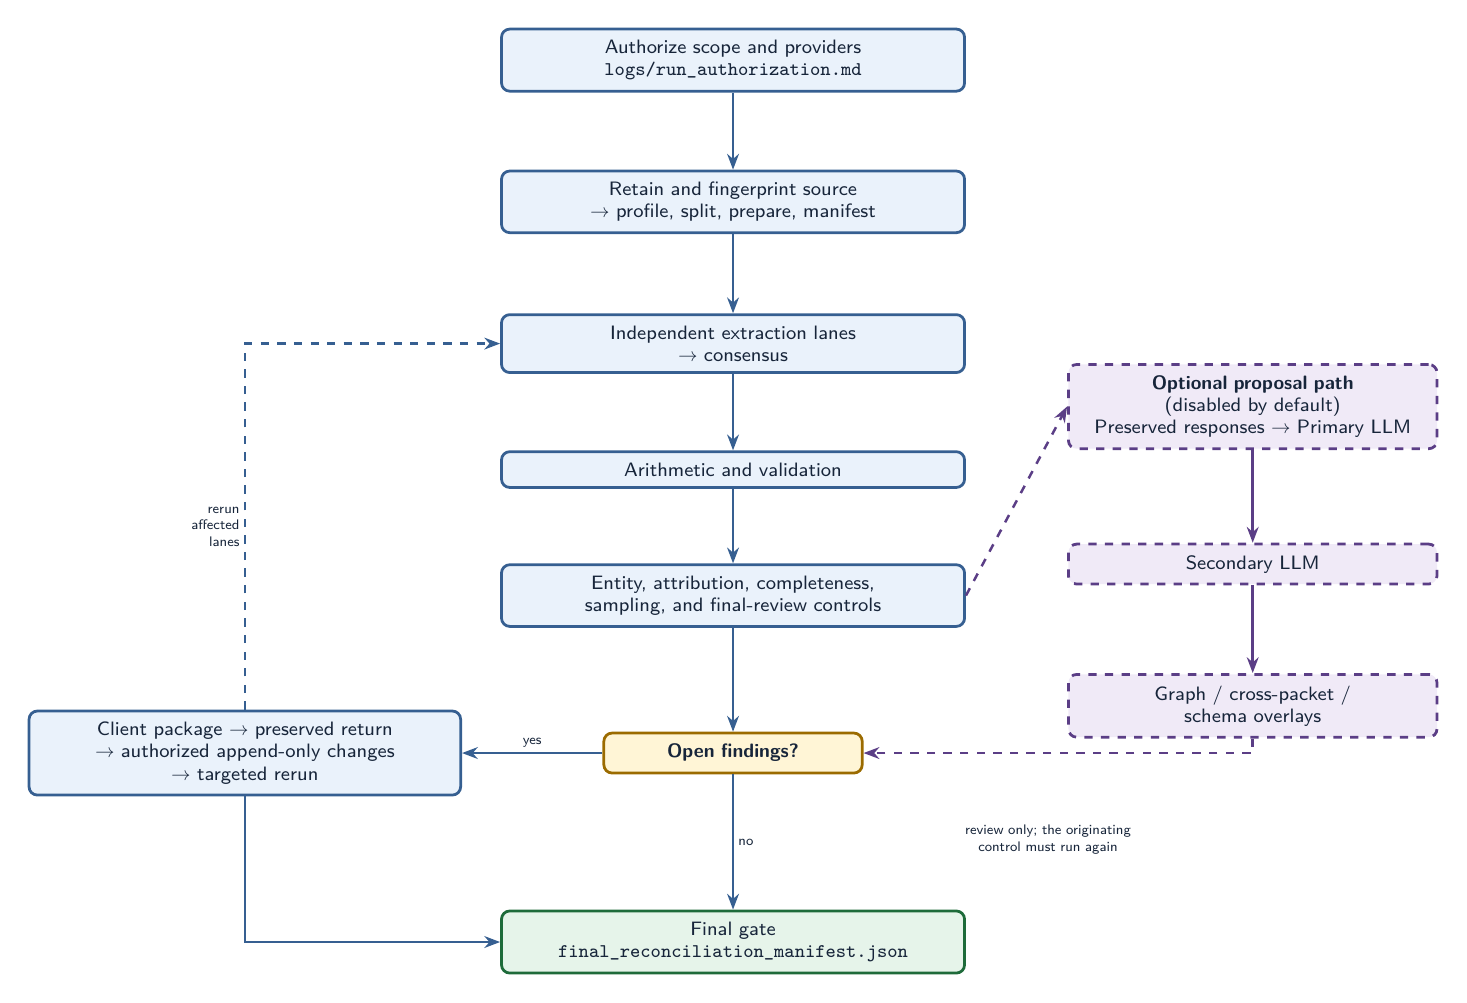
\begin{tikzpicture}[x=1mm,y=1mm]
  \node[bdi,text width=56mm] (A) at (0,0)   {Authorize scope and providers\\\texttt{logs/run\_authorization.md}};
  \node[bdi,text width=56mm] (B) at (0,-18) {Retain and fingerprint source\\$\rightarrow$ profile, split, prepare, manifest};
  \node[bdi,text width=56mm] (C) at (0,-36) {Independent extraction lanes\\$\rightarrow$ consensus};
  \node[bdi,text width=56mm] (D) at (0,-52) {Arithmetic and validation};
  \node[bdi,text width=56mm] (E) at (0,-68) {Entity, attribution, completeness,\\sampling, and final-review controls};
  \node[bdigate,text width=30mm] (F) at (0,-88) {\textbf{Open findings?}};
  \node[bdi,text width=52mm] (G) at (-62,-88) {Client package $\rightarrow$ preserved return\\$\rightarrow$ authorized append-only changes\\$\rightarrow$ targeted rerun};
  \node[bdiout,text width=56mm] (H) at (0,-112) {Final gate\\\texttt{final\_reconciliation\_manifest.json}};

  \foreach \a/\b in {A/B,B/C,C/D,D/E,E/F}{\draw[bdiflow] (\a)--(\b);}
  \draw[bdiflow] (F)--node[bdilbl,right]{no}(H);
  \draw[bdiflow] (F)--node[bdilbl,above]{yes}(G);
  \draw[bdiflow] (G.south) |- (H.west);
  % Routed up the empty left column so it crosses no control box.
  \draw[bdiback] (G.north) -- node[bdilbl,left,align=right]{rerun\\affected\\lanes}
        (G.north |- C.west) -- (C.west);

  \node[bdiopt,text width=44mm] (P1) at (66,-44) {\textbf{Optional proposal path}\\(disabled by default)\\Preserved responses $\rightarrow$ Primary LLM};
  \node[bdiopt,text width=44mm] (P2) at (66,-64) {Secondary LLM};
  \node[bdiopt,text width=44mm] (P3) at (66,-82) {Graph / cross-packet /\\schema overlays};
  \draw[bdiflow,draw=bdiOptEdge] (P1)--(P2);
  \draw[bdiflow,draw=bdiOptEdge] (P2)--(P3);
  \draw[bdiback,draw=bdiOptEdge] (E.east)--(P1.west);
  \draw[bdiback,draw=bdiOptEdge] (P3.south) |- (F.east);
  \node[bdilbl,align=center,text width=34mm] at (40,-99)
        {review only; the originating\\control must run again};
\end{tikzpicture}
}
\caption{Operating runbook control order. This is an evidence and control flow, not a data-overwrite flow; the optional proposal path adds overlays and never clears the control that raised a finding.}
\end{figure}

This is an evidence and control flow, not a data-overwrite flow. Every
optional LLM result remains a retained proposal until the normal
authorization and downstream-control path completes.

\subsection{1. Discover and authorize}\label{discover-and-authorize}

Before receiving client data, complete
\texttt{docs/\allowbreak{}CLIENT\_\allowbreak{}USER\_\allowbreak{}GUIDE.md}:

\begin{itemize}
\tightlist
\item
  source owner, transfer route, dedicated source area, and
  retention/deletion;
\item
  corpus size, date range, document families, scan characteristics, and
  known duplicate behavior;
\item
  business questions, attribution definition, GL/payment/reference
  exports;
\item
  approved providers, regions, credentials, request/cost caps, and
  caching;
\item
  golden-set design, acceptance thresholds, client reviewer, and target
  system;
\item
  whether retrieval remains local or needs separately accepted remote
  controls.
\end{itemize}

Do not begin live provider work until privacy, residency, and provider
approval are explicit.

\subsection{2. Profile, retain, split, and
prepare}\label{profile-retain-split-and-prepare}

\begin{Shaded}
\begin{Highlighting}[]
\ExtensionTok{python}\NormalTok{ scripts/scan\_profile.py SOURCE }\AttributeTok{{-}{-}out}\NormalTok{ RUN\_DIR/operations/scan\_profile.json}
\ExtensionTok{python}\NormalTok{ scripts/ingest\_pages.py SOURCE.pdf }\AttributeTok{{-}{-}out}\NormalTok{ RUN\_DIR/intake}
\ExtensionTok{python}\NormalTok{ scripts/reassemble\_pages.py RUN\_DIR/intake/ingestion\_manifest.json }\DataTypeTok{\textbackslash{}}
  \AttributeTok{{-}{-}out}\NormalTok{ RUN\_DIR/controls/reassembly.json }\DataTypeTok{\textbackslash{}}
  \AttributeTok{{-}{-}exceptions}\NormalTok{ RUN\_DIR/review/reassembly\_exceptions.json}
\ExtensionTok{python}\NormalTok{ scripts/preprocess\_pages.py RUN\_DIR/intake/pages }\DataTypeTok{\textbackslash{}}
  \AttributeTok{{-}{-}out}\NormalTok{ RUN\_DIR/preprocessing }\DataTypeTok{\textbackslash{}}
  \AttributeTok{{-}{-}manifest}\NormalTok{ RUN\_DIR/preprocessing/preprocessing\_manifest.json}
\end{Highlighting}
\end{Shaded}

The source is never modified. Inspect page counts, hashes, relative
paths, one-page boundaries, order, scan warnings, reassembly proposals,
duplicate candidates, and all classification exceptions before
extraction.

\subsection{3. Create the run manifest and
state}\label{create-the-run-manifest-and-state}

\begin{Shaded}
\begin{Highlighting}[]
\ExtensionTok{python}\NormalTok{ scripts/operations.py manifest }\DataTypeTok{\textbackslash{}}
\NormalTok{  RUN\_DIR/intake/ingestion\_manifest.json }\DataTypeTok{\textbackslash{}}
  \AttributeTok{{-}{-}config{-}from{-}env} \AttributeTok{{-}{-}out}\NormalTok{ RUN\_DIR/operations/run\_manifest.json}
\ExtensionTok{python}\NormalTok{ scripts/operations.py stage RUN\_DIR/operations/run\_state.json profile }\DataTypeTok{\textbackslash{}}
  \AttributeTok{{-}{-}manifest{-}hash}\NormalTok{ MANIFEST\_SHA256}
\ExtensionTok{python}\NormalTok{ scripts/operations.py stage RUN\_DIR/operations/run\_state.json intake }\DataTypeTok{\textbackslash{}}
  \AttributeTok{{-}{-}manifest{-}hash}\NormalTok{ MANIFEST\_SHA256}
\end{Highlighting}
\end{Shaded}

Keep the manifest hash constant for resumed stages. A changed input or
effective configuration requires a new run.

\subsection{4. Produce independent extraction
evidence}\label{produce-independent-extraction-evidence}

Invoke the primary and secondary lanes separately:

\begin{Shaded}
\begin{Highlighting}[]
\ExtensionTok{python}\NormalTok{ scripts/llm\_adapter.py RUN\_DIR/intake/ingestion\_manifest.json }\DataTypeTok{\textbackslash{}}
  \AttributeTok{{-}{-}lane}\NormalTok{ consensus\_primary }\DataTypeTok{\textbackslash{}}
  \AttributeTok{{-}{-}out}\NormalTok{ RUN\_DIR/providers/primary\_engine.json }\DataTypeTok{\textbackslash{}}
  \AttributeTok{{-}{-}adapter{-}out}\NormalTok{ RUN\_DIR/providers/primary\_handoff.json }\DataTypeTok{\textbackslash{}}
  \AttributeTok{{-}{-}exceptions}\NormalTok{ RUN\_DIR/review/primary\_exceptions.json }\DataTypeTok{\textbackslash{}}
  \AttributeTok{{-}{-}raw{-}dir}\NormalTok{ RUN\_DIR/providers/primary\_raw}

\ExtensionTok{python}\NormalTok{ scripts/llm\_adapter.py RUN\_DIR/intake/ingestion\_manifest.json }\DataTypeTok{\textbackslash{}}
  \AttributeTok{{-}{-}lane}\NormalTok{ consensus\_secondary }\DataTypeTok{\textbackslash{}}
  \AttributeTok{{-}{-}out}\NormalTok{ RUN\_DIR/providers/secondary\_engine.json }\DataTypeTok{\textbackslash{}}
  \AttributeTok{{-}{-}adapter{-}out}\NormalTok{ RUN\_DIR/providers/secondary\_handoff.json }\DataTypeTok{\textbackslash{}}
  \AttributeTok{{-}{-}exceptions}\NormalTok{ RUN\_DIR/review/secondary\_exceptions.json }\DataTypeTok{\textbackslash{}}
  \AttributeTok{{-}{-}raw{-}dir}\NormalTok{ RUN\_DIR/providers/secondary\_raw}
\end{Highlighting}
\end{Shaded}

The two lane providers must be genuinely independent. Validate each
adapter handoff and retain every raw response and exception. Two empty
or failed engine records are never agreement.

For source-native tables, follow
\texttt{references/\allowbreak{}table-\allowbreak{}comprehension.md}.
Profile layout, propose source rows with cell evidence, run the
non-independent audit, optionally invoke Document AI for a conditional
buddy audit, then map only with an exact client-approved registry.
Corpus refinement is sequential because source-layout context is
order-dependent. Every changed reread is a linked amendment proposal.

\subsection{5. Reconcile and validate}\label{reconcile-and-validate}

\begin{Shaded}
\begin{Highlighting}[]
\ExtensionTok{python}\NormalTok{ scripts/consensus.py }\DataTypeTok{\textbackslash{}}
\NormalTok{  RUN\_DIR/providers/primary\_engine.json }\DataTypeTok{\textbackslash{}}
\NormalTok{  RUN\_DIR/providers/secondary\_engine.json }\DataTypeTok{\textbackslash{}}
  \AttributeTok{{-}{-}out}\NormalTok{ RUN\_DIR/controls/consensus.json }\DataTypeTok{\textbackslash{}}
  \AttributeTok{{-}{-}exceptions}\NormalTok{ RUN\_DIR/review/consensus\_exceptions.json}
\ExtensionTok{python}\NormalTok{ scripts/arithmetic\_check.py RUN\_DIR/controls/consensus.json }\DataTypeTok{\textbackslash{}}
  \AttributeTok{{-}{-}out}\NormalTok{ RUN\_DIR/controls/proofed.json}
\ExtensionTok{python}\NormalTok{ scripts/adjudicate.py RUN\_DIR/controls/proofed.json }\DataTypeTok{\textbackslash{}}
\NormalTok{  RUN\_DIR/providers/primary\_engine.json }\DataTypeTok{\textbackslash{}}
\NormalTok{  RUN\_DIR/providers/secondary\_engine.json }\DataTypeTok{\textbackslash{}}
  \AttributeTok{{-}{-}out}\NormalTok{ RUN\_DIR/review/amendment\_proposals.json }\DataTypeTok{\textbackslash{}}
  \AttributeTok{{-}{-}exceptions}\NormalTok{ RUN\_DIR/review/adjudication\_exceptions.json}
\ExtensionTok{python}\NormalTok{ scripts/validate\_extraction.py RUN\_DIR/controls/proofed.json }\DataTypeTok{\textbackslash{}}
  \AttributeTok{{-}{-}out}\NormalTok{ RUN\_DIR/controls/validated.json }\DataTypeTok{\textbackslash{}}
  \AttributeTok{{-}{-}exceptions}\NormalTok{ RUN\_DIR/review/validation\_exceptions.json}
\end{Highlighting}
\end{Shaded}

Consensus accepts only
\texttt{independent\_\allowbreak{}extraction\_\allowbreak{}handoff\_\allowbreak{}v1}
artifacts from distinct provider groups and consensus lanes. It verifies
embedded record and retained raw-response hashes, compares typed values
without coercing identifiers into numbers, rejects duplicate
engine/document records, and carries a voted document type or
\texttt{unknown}. Arithmetic compares source-visible equations within
the configured absolute tolerance. Adjudication is bounded and
amendment-only. Validation never silently normalizes a failed field into
passing status.

\subsubsection{Source-template
observations}\label{source-template-observations}

Three lanes read a source-template observation artifact and nothing else
produces one: \texttt{schema\_\allowbreak{}discovery.py discover},
\texttt{allocation\_\allowbreak{}policy.py discover}, and
\texttt{template\_\allowbreak{}drift.py analyze}. Build it here, from
the completed consensus run, or those lanes cannot run at all.

\begin{Shaded}
\begin{Highlighting}[]
\ExtensionTok{python}\NormalTok{ scripts/template\_observations.py RUN\_DIR/controls/consensus.json }\DataTypeTok{\textbackslash{}}
  \AttributeTok{{-}{-}out}\NormalTok{ RUN\_DIR/templates/observed\_templates.json }\DataTypeTok{\textbackslash{}}
  \AttributeTok{{-}{-}exceptions}\NormalTok{ RUN\_DIR/templates/observed\_template\_exceptions.json}
\end{Highlighting}
\end{Shaded}

A template is one document family, not one page. Labels are the union of
what a family's documents showed, each carrying the number of documents
it appeared in, so capture variance stays visible instead of producing
one template per page. Labels are copied exactly as printed and ordered
deterministically rather than in layout order, so drift detection sees
an added or removed label and not a reordering. Nothing here is a
mapping.

This is also why template drift is computed after consensus rather than
in Phase 2: its input does not exist until extraction has run. A changed
vendor layout is therefore detected after that layout has been
extracted.

\subsection{6. Run business controls}\label{run-business-controls}

\begin{Shaded}
\begin{Highlighting}[]
\ExtensionTok{python}\NormalTok{ scripts/address\_normalize.py RUN\_DIR/controls/validated.json }\DataTypeTok{\textbackslash{}}
  \AttributeTok{{-}{-}out}\NormalTok{ RUN\_DIR/controls/address\_normalized.json }\DataTypeTok{\textbackslash{}}
  \AttributeTok{{-}{-}exceptions}\NormalTok{ RUN\_DIR/review/address\_exceptions.json}
\ExtensionTok{python}\NormalTok{ scripts/entity\_resolve.py RUN\_DIR/controls/address\_normalized.json }\DataTypeTok{\textbackslash{}}
  \AttributeTok{{-}{-}out}\NormalTok{ RUN\_DIR/controls/parties.json }\DataTypeTok{\textbackslash{}}
  \AttributeTok{{-}{-}log}\NormalTok{ RUN\_DIR/controls/entity\_merges.json}
\ExtensionTok{python}\NormalTok{ scripts/attribution.py RUN\_DIR/controls/proofed.json }\DataTypeTok{\textbackslash{}}
  \AttributeTok{{-}{-}reference}\NormalTok{ REFERENCE\_EXPORT }\DataTypeTok{\textbackslash{}}
  \AttributeTok{{-}{-}out}\NormalTok{ RUN\_DIR/controls/attributed.json }\DataTypeTok{\textbackslash{}}
  \AttributeTok{{-}{-}register}\NormalTok{ RUN\_DIR/review/unattributable.json}
\ExtensionTok{python}\NormalTok{ scripts/completeness.py RUN\_DIR/controls/attributed.json }\DataTypeTok{\textbackslash{}}
  \AttributeTok{{-}{-}gl}\NormalTok{ GL\_EXPORT }\AttributeTok{{-}{-}payments}\NormalTok{ PAYMENT\_EXPORT }\DataTypeTok{\textbackslash{}}
  \AttributeTok{{-}{-}out}\NormalTok{ RUN\_DIR/controls/completeness.json}
\ExtensionTok{python}\NormalTok{ scripts/sampling.py RUN\_DIR/controls/attributed.json }\DataTypeTok{\textbackslash{}}
  \AttributeTok{{-}{-}materiality}\NormalTok{ MATERIALITY }\AttributeTok{{-}{-}out}\NormalTok{ RUN\_DIR/controls/sample\_plan.json}
\end{Highlighting}
\end{Shaded}

Name the client with
\texttt{entity\_\allowbreak{}resolve.py -\allowbreak{}-\allowbreak{}client-\allowbreak{}name},
as the pages print it, or the client becomes its own largest
counterparty. Give \texttt{-\/-party-decisions} a person's decisions
about named pairs -- \texttt{same\_\allowbreak{}party},
\texttt{branch\_\allowbreak{}of} (both accounts kept, the branch linked
to its parent), \texttt{different\_\allowbreak{}parties} and
\texttt{not\_\allowbreak{}a\_\allowbreak{}party} -- under the
authorization the file names. A decided pair leaves pending adjudication
with its score kept, and a decision the resolver cannot apply is
reported with its reason rather than guessed at.

\subsubsection{Recovering a printed column the schema had no field
for}\label{recovering-a-printed-column-the-schema-had-no-field-for}

A schema that names no home for a printed column does not make an engine
skip it: the value goes into whichever field looks closest, both vendors
pick the same one, and it arrives accepted. Before proposing a
re-extraction to capture such a column, reconcile from what the run
already retains. Every provider response is kept, and the independent
non-LLM extractor retains the whole page rather than the fields the
schema asked for.

\begin{Shaded}
\begin{Highlighting}[]
\ExtensionTok{python}\NormalTok{ scripts/specifier\_recover.py RUN\_DIR/controls/validated.json }\DataTypeTok{\textbackslash{}}
  \AttributeTok{{-}{-}extractor{-}raw}\NormalTok{ RUN\_DIR/providers/raw/docai }\DataTypeTok{\textbackslash{}}
  \AttributeTok{{-}{-}out}\NormalTok{ RUN\_DIR/controls/records\_with\_specifiers.json }\DataTypeTok{\textbackslash{}}
  \AttributeTok{{-}{-}exceptions}\NormalTok{ RUN\_DIR/review/specifier\_recovery\_exceptions.json}
\end{Highlighting}
\end{Shaded}

The join is a printed key both sides already carry -- these forms group
lines under a header reading COMPANY / ACK\# / P.O.\# / P.O. DATE /
SPECIFIER, so the specifier printed beside a purchase-order number
belongs to every line quoting it. A recovered reading is one extractor
with no model behind it, so it is written unaccepted as a single reading
and never carries the corroboration status that pairs a model with an
extractor. A line already stating a specifier keeps its own, and a page
printing a specifier no line claims yields an exception rather than a
guess.

Every lane reading the extractor's pages indexes them through
\texttt{run\_\allowbreak{}io.retained\_\allowbreak{}responses}, which
takes the response that read the page. A request that came back without
text is retried and both files are kept, and on the commission run 222
of 716 pages had text only in the retry: indexing the first file per
page left all 222 empty to brand recovery, to this lane and to the page
review's extractor evidence.

\texttt{brand\_\allowbreak{}recover.py} recovers the manufacturer the
same way, from the retained page rather than a new call. It reads the
letterhead first -- the name at the top wins when a letterhead names
two, and a name of ten letters or more may be read one letter off --
then gives a page naming no maker the one its opening shares with that
maker's other pages. A continuation page prints its maker's columns and
none of its letterhead, so a page still unsettled takes the maker only
whose settled pages print at least three of its words, or else the maker
every one of its five most alike settled pages names. A page whose top
names a company by its legal form, neither the client nor a known maker,
stays an exception naming that company: Crestline Design's
funds-transfer advices read like Marlow/Bramwell's bill payments, and a
test over the pages the vocabulary already knows cannot see a maker it
lacks.

After reviewing every certainty and MUS selection, provide a
\texttt{sample\_\allowbreak{}review\_\allowbreak{}results\_\allowbreak{}v1}
artifact containing the plan's
\texttt{sample\_\allowbreak{}plan\_\allowbreak{}sha256} and exactly one
explicit outcome per selected document. Missing, duplicate, foreign,
stale, abstained, failed, or contradictory outcomes block the accuracy
statement; an empty file is never a zero-error result.

Address processing is local unless Google Address Validation is
explicitly enabled. Provider results add derived evidence and never
replace the raw address. Entity merges are reversible. Attribution
enumerates every unresolved in-scope dollar. Completeness blocks on
missing or unmeasurable reconciliation inputs, out-of-tolerance periods,
unresolved/ambiguous payments, sequence or calendar gaps, and undated
documents.

Run \texttt{handwriting\_\allowbreak{}review.py} only with independent
HTR results. Printed and handwritten evidence remain separate.
Handwritten financial readings require strict reconciliation and still
become review-required amendments.

The optional Google handwriting lane uses Cloud Vision's
handwriting-capable
\texttt{DOCUMENT\_\allowbreak{}TEXT\_\allowbreak{}DETECTION} feature on
every retained page. Supply one or more separately produced
extraction/profile artifacts containing normalized
\texttt{handwriting\_\allowbreak{}regions}; Google reads those regions
but does not prove that its own reading is correct:

\begin{Shaded}
\begin{Highlighting}[]
\ExtensionTok{python}\NormalTok{ scripts/google\_handwriting\_ocr.py }\DataTypeTok{\textbackslash{}}
\NormalTok{  RUN\_DIR/intake/ingestion\_manifest.json }\DataTypeTok{\textbackslash{}}
  \AttributeTok{{-}{-}regions}\NormalTok{ RUN\_DIR/extraction/primary\_records.json }\DataTypeTok{\textbackslash{}}
  \AttributeTok{{-}{-}out}\NormalTok{ RUN\_DIR/handwriting/google\_htr.json }\DataTypeTok{\textbackslash{}}
  \AttributeTok{{-}{-}adapter{-}out}\NormalTok{ RUN\_DIR/handwriting/google\_htr\_adapter.json }\DataTypeTok{\textbackslash{}}
  \AttributeTok{{-}{-}exceptions}\NormalTok{ RUN\_DIR/handwriting/google\_htr\_exceptions.json }\DataTypeTok{\textbackslash{}}
  \AttributeTok{{-}{-}raw{-}dir}\NormalTok{ RUN\_DIR/handwriting/google\_htr\_raw }\DataTypeTok{\textbackslash{}}
  \AttributeTok{{-}{-}images{-}dir}\NormalTok{ RUN\_DIR/handwriting/google\_htr\_pages }\AttributeTok{{-}{-}enable}
\end{Highlighting}
\end{Shaded}

Every page receives one success/failure record. A page without a
supplied region is recorded as OCR-complete but not declared
handwriting-free. Freeze the raw response and rendered-page directories.
Retry provider failures in a new directory, then reconcile the resulting
\texttt{google\_\allowbreak{}htr.json} with genuinely separate HTR
provider groups. The other inputs may be HTR annotation artifacts or
retained visual-extraction record lists; each region/reading pair must
share the same stable \texttt{region\_\allowbreak{}id}:

\begin{Shaded}
\begin{Highlighting}[]
\ExtensionTok{python}\NormalTok{ scripts/handwriting\_review.py }\DataTypeTok{\textbackslash{}}
\NormalTok{  RUN\_DIR/handwriting/google\_htr.json }\DataTypeTok{\textbackslash{}}
\NormalTok{  RUN\_DIR/extraction/openai\_records.json OTHER\_PROVIDER\_HTR.json }\DataTypeTok{\textbackslash{}}
  \AttributeTok{{-}{-}out}\NormalTok{ RUN\_DIR/handwriting/decisions.json }\DataTypeTok{\textbackslash{}}
  \AttributeTok{{-}{-}exceptions}\NormalTok{ RUN\_DIR/handwriting/exceptions.json}
\end{Highlighting}
\end{Shaded}

Three independent groups must unanimously agree on handwritten numerics;
two independent groups suffice for free text. Same-provider models and
prompt roles count once. Signatures and financial amendments remain
review work.

\subsection{7. Build and reduce the review surface
safely}\label{build-and-reduce-the-review-surface-safely}

Three options here are omissions rather than refinements, and each fails
quietly. \texttt{-\/-resolved-by} retains a document-type proposal the
run already answered instead of asking it again; without it a real
corpus re-asked 1,121 settled questions. \texttt{-\/-classifications}
gives grouping the document type the extraction consensus declined to
claim -- it writes \texttt{"unknown"} wherever its lanes could not
agree, which was 691 of 718 documents on a real corpus, and without the
classification artifact those become one undifferentiated
\texttt{unclassified\_\allowbreak{}document\_\allowbreak{}family} group
and the family is guessed from words in the reason string. The pack lane
needs both, because it builds the same queue by its own path.

\begin{Shaded}
\begin{Highlighting}[]
\ExtensionTok{python}\NormalTok{ scripts/final\_review\_queue.py RUN\_DIR/review/}\PreprocessorTok{*}\NormalTok{.json }\DataTypeTok{\textbackslash{}}
\NormalTok{  RUN\_DIR/controls/validated.json }\DataTypeTok{\textbackslash{}}
\NormalTok{  RUN\_DIR/controls/completeness.json }\DataTypeTok{\textbackslash{}}
  \AttributeTok{{-}{-}resolved{-}by}\NormalTok{ RUN\_DIR/controls/classification\_consensus.json }\DataTypeTok{\textbackslash{}}
  \AttributeTok{{-}{-}out}\NormalTok{ RUN\_DIR/review/final\_client\_review.json}
\ExtensionTok{python}\NormalTok{ scripts/review\_grouping.py RUN\_DIR/review/final\_client\_review.json }\DataTypeTok{\textbackslash{}}
  \AttributeTok{{-}{-}consensus}\NormalTok{ RUN\_DIR/controls/consensus.json }\DataTypeTok{\textbackslash{}}
  \AttributeTok{{-}{-}classifications}\NormalTok{ RUN\_DIR/controls/classification\_consensus.json }\DataTypeTok{\textbackslash{}}
  \AttributeTok{{-}{-}out}\NormalTok{ RUN\_DIR/review/grouping.json}
\ExtensionTok{python}\NormalTok{ scripts/client\_review\_lane.py build RUN\_DIR/review/}\PreprocessorTok{*}\NormalTok{.json }\DataTypeTok{\textbackslash{}}
  \AttributeTok{{-}{-}consensus}\NormalTok{ RUN\_DIR/controls/consensus.json }\DataTypeTok{\textbackslash{}}
  \AttributeTok{{-}{-}classifications}\NormalTok{ RUN\_DIR/controls/classification\_consensus.json }\DataTypeTok{\textbackslash{}}
  \AttributeTok{{-}{-}resolved{-}by}\NormalTok{ RUN\_DIR/controls/classification\_consensus.json }\DataTypeTok{\textbackslash{}}
  \AttributeTok{{-}{-}manifest}\NormalTok{ RUN\_DIR/pages/ingestion\_manifest.json }\DataTypeTok{\textbackslash{}}
  \AttributeTok{{-}{-}out{-}dir}\NormalTok{ RUN\_DIR/review/client\_pack\_01}
\ExtensionTok{python}\NormalTok{ scripts/operations.py review{-}export }\DataTypeTok{\textbackslash{}}
\NormalTok{  RUN\_DIR/review/final\_client\_review.json }\DataTypeTok{\textbackslash{}}
  \AttributeTok{{-}{-}csv}\NormalTok{ RUN\_DIR/review/final\_client\_review.csv }\DataTypeTok{\textbackslash{}}
  \AttributeTok{{-}{-}html}\NormalTok{ RUN\_DIR/review/final\_client\_review.html }\DataTypeTok{\textbackslash{}}
  \AttributeTok{{-}{-}xlsx}\NormalTok{ RUN\_DIR/review/final\_client\_review.xlsx}
\end{Highlighting}
\end{Shaded}

The JSON queue is authoritative. CSV, HTML, and XLSX are reviewer aids.
The card-level reviewer, cross-record pass, full-dataset agent,
grouping, and safe consolidation are optional and disabled by default.
They retain the original queue and may reduce only the client-facing
presentation of explicitly eligible low-risk dependencies.

All review-reduction paths use the shared fail-closed protected-item
taxonomy. Unknown reason codes are protected. Cross-record proof must
come through the strict
\texttt{cross\_\allowbreak{}record\_\allowbreak{}evidence\_\allowbreak{}v1}
envelope and one exact versioned producer handoff.
\texttt{intake\_\allowbreak{}evidence\_\allowbreak{}producer\_\allowbreak{}v1}
binds the complete intake manifest, classification-exception artifact,
retained source/page/text files, and operations manifest. The reducer
reruns the retained deterministic text extraction and classifier and
admits only rule-classified
\texttt{pages[].document\_\allowbreak{}type}.
\texttt{canonical\_\allowbreak{}evidence\_\allowbreak{}producer\_\allowbreak{}v1}
binds the exact canonical export to its checksummed load plan, clear
final-review artifact, source PDFs, and operations manifest; only
\texttt{tables.document[].document\_\allowbreak{}type} is eligible.
Extra semantic fields, self-labelled tuples, arbitrary JSON, malformed
entries, raw/provider update fields, suggestions, and unresolved or
non-clear facts are reported as ineligible context.

Evidence preflight is local and precedes provider I/O. By default each
envelope or required producer/source artifact is capped at 10,000,000
bytes and the supplied collection is capped at 10,000 declared entries.
Positive overrides are available through
\texttt{-\/-max-evidence-artifact-bytes},
\texttt{-\/-max-evidence-entries}, and their documented environment
settings. A breach emits an explicit review exception without a provider
call. The reducer first size-bounds and parses every envelope and totals
all declared entries; no producer is loaded when the aggregate limit
fails. Every producer, handoff, source PDF, page PDF, and retained text
file is size-checked before its first hash, open, or read. Producer
indexes are built once; authenticated source hashes, PDF validity, and
page counts are cached so repeated entries read and open each retained
source once. Even an empty collection reports an invalid producer once
at \texttt{\$.producer}; for a non-empty invalid producer, every
declared entry is separately retained, with otherwise valid entries
marked \texttt{producer\_\allowbreak{}not\_\allowbreak{}authenticated}.

A proposed update must target the reviewed field, use exact non-empty
whitespace-free target and different source identities, pass finite
non-Boolean \texttt{{[}0,\ 1{]}} confidence validation, and resolve one
entry. Every failure remains review work with a machine reason. Eligible
updates remain proposal-only and record the exact envelope, producer,
and source provenance. Protected findings, including provider/schema,
arithmetic, reassembly, handwriting, identity, review-flag,
missing-field, and unresolved-evidence items, cannot be batch cleared.

When authorized and calibrated, run
\texttt{safe\_\allowbreak{}review\_\allowbreak{}consolidation.py} into a
fresh directory. With grouping enabled it generates the small
reproducible workbook, plain-language guide, decision pages, and ZIP.
The package intentionally has no client appendix or drill-down; the
internal JSON retains the exhaustive detail.

\subsection{8. Process a returned client
workbook}\label{process-a-returned-client-workbook}

Preserve the issued workbook and the returned copy separately. Import
them together:

\begin{Shaded}
\begin{Highlighting}[]
\ExtensionTok{python}\NormalTok{ scripts/client\_review\_package.py import{-}decisions }\DataTypeTok{\textbackslash{}}
\NormalTok{  RETURNED.xlsx }\AttributeTok{{-}{-}issued{-}workbook}\NormalTok{ ISSUED.xlsx }\DataTypeTok{\textbackslash{}}
  \AttributeTok{{-}{-}out}\NormalTok{ RUN\_DIR/review/client\_decisions.json}
\end{Highlighting}
\end{Shaded}

The importer validates package structure, hidden safe-consolidation
lineage, group completeness/order, fixed cells, controlled choices,
protected decisions, editable columns, notes for client-supplied
alternatives, ZIP safety limits, and both workbook hashes. Its output is
proposal-only.

If the returned workbook is legacy or otherwise blocked by lineage,
preserve the exact client choices and notes before troubleshooting the
package:

\begin{Shaded}
\begin{Highlighting}[]
\ExtensionTok{python}\NormalTok{ scripts/client\_review\_package.py preserve{-}responses }\DataTypeTok{\textbackslash{}}
\NormalTok{  RETURNED.xlsx }\AttributeTok{{-}{-}issued{-}workbook}\NormalTok{ ISSUED.xlsx }\DataTypeTok{\textbackslash{}}
  \AttributeTok{{-}{-}out}\NormalTok{ RUN\_DIR/review/client\_responses\_preserved.json}
\end{Highlighting}
\end{Shaded}

This no-clobber, proposal-only artifact records every decision row,
response count, workbook hashes, fixed-cell comparison, and any lineage
exception. It does not alter either workbook and should accompany any
reissued package.

When an authoritative client reference, GL, or payment export is
missing, keep that control explicitly blocked. An operator may create a
separate, hash-bound proposal package to prioritize follow-up, but it
cannot turn the completeness gate clear:

\begin{Shaded}
\begin{Highlighting}[]
\ExtensionTok{python}\NormalTok{ scripts/inferred\_controls.py RUN\_DIR/controls/consensus\_or\_proofed.json }\DataTypeTok{\textbackslash{}}
  \AttributeTok{{-}{-}out{-}dir}\NormalTok{ RUN\_DIR/review/inferred\_controls\_proposal}
\end{Highlighting}
\end{Shaded}

For bounded post-return reference reasoning, first construct context
from the preserved response artifact and a deterministic selection of
retained records:

\begin{Shaded}
\begin{Highlighting}[]
\ExtensionTok{python}\NormalTok{ scripts/client\_review\_context.py }\DataTypeTok{\textbackslash{}}
\NormalTok{  RUN\_DIR/review/client\_responses\_preserved.json }\DataTypeTok{\textbackslash{}}
  \AttributeTok{{-}{-}records}\NormalTok{ RUN\_DIR/controls/consensus\_or\_proofed.json }\DataTypeTok{\textbackslash{}}
  \AttributeTok{{-}{-}out}\NormalTok{ RUN\_DIR/review/client\_review\_context.json}
\end{Highlighting}
\end{Shaded}

If the client supplied comments outside the returned workbook, parse one
or more general comment files into the same context contract, then
include the result in source-native corpus forward and refinement calls:

\begin{Shaded}
\begin{Highlighting}[]
\ExtensionTok{python}\NormalTok{ scripts/client\_input\_comments.py client\_notes.json client\_followup.csv }\DataTypeTok{\textbackslash{}}
  \AttributeTok{{-}{-}out}\NormalTok{ RUN\_DIR/review/client\_input\_comments\_context.json}
\ExtensionTok{python}\NormalTok{ scripts/table\_comprehension\_corpus.py }\DataTypeTok{\textbackslash{}}
\NormalTok{  RUN\_DIR/intake/ingestion\_manifest.json }\DataTypeTok{\textbackslash{}}
  \AttributeTok{{-}{-}client{-}context}\NormalTok{ RUN\_DIR/review/client\_input\_comments\_context.json }\DataTypeTok{\textbackslash{}}
  \AttributeTok{{-}{-}out}\NormalTok{ RUN\_DIR/tables/corpus\_with\_client\_context}
\end{Highlighting}
\end{Shaded}

JSON may be a list or an object containing \texttt{comments{[}{]}};
CSV/TSV requires a \texttt{client\_\allowbreak{}comment},
\texttt{comment}, \texttt{comments}, \texttt{note}, or \texttt{text}
column; TXT and Markdown preserve each non-empty line. Every comment and
source field remains verbatim and hash-bound. It may guide terminology,
priorities, and questions, but cannot supply document facts, independent
consensus, authorization, or control clearance. The context hash is part
of resumable corpus identity.

The context marks every client comment as reasoning-only and excludes it
from independent consensus. The legacy one-pass discovery lane
(\texttt{client\_\allowbreak{}review\_\allowbreak{}inference.py}) and
the preferred iterative lane are both disabled unless explicitly
invoked. The iterative lane uses a configured Primary LLM and
independently configured Secondary LLM, retains raw responses and a
record-level exception for any item that cannot fit its bounded packet,
and accepts the full retained corpus only through \texttt{-\/-records}:

\begin{Shaded}
\begin{Highlighting}[]
\ExtensionTok{python}\NormalTok{ scripts/client\_review\_iterative.py }\DataTypeTok{\textbackslash{}}
\NormalTok{  RUN\_DIR/review/client\_review\_context.json }\DataTypeTok{\textbackslash{}}
  \AttributeTok{{-}{-}primary{-}out}\NormalTok{ RUN\_DIR/review/iterative\_primary.json }\DataTypeTok{\textbackslash{}}
  \AttributeTok{{-}{-}buddy{-}out}\NormalTok{ RUN\_DIR/review/iterative\_buddy.json }\DataTypeTok{\textbackslash{}}
  \AttributeTok{{-}{-}exceptions}\NormalTok{ RUN\_DIR/review/iterative\_exceptions.json }\DataTypeTok{\textbackslash{}}
  \AttributeTok{{-}{-}raw{-}dir}\NormalTok{ RUN\_DIR/review/iterative\_raw }\DataTypeTok{\textbackslash{}}
  \AttributeTok{{-}{-}records}\NormalTok{ RUN\_DIR/controls/consensus\_or\_proofed.json }\AttributeTok{{-}{-}iterations}\NormalTok{ 3 }\DataTypeTok{\textbackslash{}}
  \AttributeTok{{-}{-}convergence{-}min{-}new{-}candidates}\NormalTok{ 1}
\end{Highlighting}
\end{Shaded}

The lane adapts serialized packet boundaries and reserves 40,000 bytes
for instructions, carried proposals, and buddy decisions; it retains
every raw request and response, and writes exact
\texttt{source\_\allowbreak{}document\_\allowbreak{}ids} into every
exhausted batch exception. Retries are bounded; recovery uses a
separate, no-clobber retry run for the named records, and any residual
remains explicit review work. Its \texttt{confirmed} and
\texttt{close\_\allowbreak{}needs\_\allowbreak{}review} states are still
source-linked proposals only. They cannot establish GL/payment facts,
approve attribution, clear completeness, or authorize a canonical fact.
Build the deterministic JSON evidence graph from the selected,
hash-bound artifacts when graph queries will help a reviewer; its
\texttt{build}, \texttt{query}, \texttt{path}, \texttt{candidates},
\texttt{contradictions}, \texttt{schema}, and \texttt{schema-surface}
commands preserve evidence and conflicts rather than resolve them. The
bounded \texttt{schema} inventory reports observed field names, counts,
examples, and claim provenance for proposal-only schema discovery.
\texttt{schema-surface} reads an exact retained consensus artifact and
separately reports non-consensus candidate fields, source pointers, and
label-bound address/contact/representative signals. It retains all raw
signals and provides only a bounded, source-cited signal summary to
schema discovery; it never turns a candidate into a graph fact or
canonical mapping. See
\texttt{references/\allowbreak{}artifact-\allowbreak{}contracts.md} and
\texttt{references/\allowbreak{}command-\allowbreak{}line-\allowbreak{}reference.md}
for the exact artifact manifest and CLI contracts.

The extraction contract has a broad controlled core for commercial
references, party/contact roles, payment/tax, sales, commission, and
logistics fields. It also requires a source-labelled extension record
for every other visible labeled value. This gives unfamiliar document
families a retained, source-cited path into schema review instead of
discarding an out-of-vocabulary field. The extension is proposal-only: a
later mapping still needs evidence and approval.

The iterative primary/buddy provider, model, optional
credential-variable override, timeout, retry, backoff, reasoning effort,
and packet limits are all read from \texttt{.env} and recorded in the
outputs. The code rejects a missing model, unsupported provider, or
matching primary/buddy provider before provider I/O; safe code
validation never silently selects a provider for a production run.

To propose next steps for retained reassembly, validation, or
attribution exceptions, use the separate disabled-by-default
control-exception lane. It receives immutable records, named control
findings, and---when client feedback is available---the preserved
\texttt{client\_\allowbreak{}review\_\allowbreak{}context\_\allowbreak{}v1}
as reasoning-only context. It uses configured independent primary and
buddy providers, preserves raw responses, and never changes the source
records or clears a gate:

\begin{Shaded}
\begin{Highlighting}[]
\ExtensionTok{python}\NormalTok{ scripts/client\_review\_exception\_resolution.py }\DataTypeTok{\textbackslash{}}
\NormalTok{  RUN\_DIR/controls/consensus\_or\_proofed.json }\DataTypeTok{\textbackslash{}}
  \AttributeTok{{-}{-}exceptions}\NormalTok{ RUN\_DIR/controls/arithmetic.json }\DataTypeTok{\textbackslash{}}
  \AttributeTok{{-}{-}exceptions}\NormalTok{ RUN\_DIR/controls/validation\_exceptions.json }\DataTypeTok{\textbackslash{}}
  \AttributeTok{{-}{-}exceptions}\NormalTok{ RUN\_DIR/controls/attribution\_register.json }\DataTypeTok{\textbackslash{}}
  \AttributeTok{{-}{-}client{-}context}\NormalTok{ RUN\_DIR/review/client\_review\_context.json }\DataTypeTok{\textbackslash{}}
  \AttributeTok{{-}{-}out}\NormalTok{ RUN\_DIR/review/exception\_resolution\_proposals.json }\DataTypeTok{\textbackslash{}}
  \AttributeTok{{-}{-}exceptions{-}out}\NormalTok{ RUN\_DIR/review/exception\_resolution\_exceptions.json }\DataTypeTok{\textbackslash{}}
  \AttributeTok{{-}{-}raw{-}dir}\NormalTok{ RUN\_DIR/review/exception\_resolution\_raw }\AttributeTok{{-}{-}enable}
\end{Highlighting}
\end{Shaded}

This lane uses the shared serialized-byte adaptive packet utility. It
combines all supplied findings for one source record, reduces packet
size before provider I/O, and records any individually oversized record
or positive batch-cap remainder explicitly. It rejects duplicate record
IDs, accounts for findings whose source record is absent, and gives the
buddy reviewer the same findings, source records, and reasoning-only
client context as the primary reviewer. A primary proposal is retained
as rejected if its document or related-document ID falls outside the
packet or its evidence quote is not present in the compact source
packet. Review and apply only eligible append-only proposals, then rerun
reassembly, arithmetic, validation, attribution, completeness, and final
review. Inferred document evidence cannot clear authoritative GL or
payment/remittance reconciliation. Every input finding has an exception
ID, and every retained proposal names the source exception IDs it
addresses so later overlays can be reconciled without guessing from
batch membership. Provider/schema failures, individually oversized work,
and cap-deferred work also retain the exact original findings, control
kinds, and exception IDs. Passing that companion exception artifact to a
new no-clobber recovery therefore reconstructs the original control
packet rather than substituting a generic provider-failure finding or
guessing from document membership.

\subsubsection{AI simulated-client review
comments}\label{ai-simulated-client-review-comments}

\texttt{scripts/\allowbreak{}ai\_\allowbreak{}simulated\_\allowbreak{}client\_\allowbreak{}review.py}
is intentionally separate from both the client workbook import and the
client-review reduction lane. It accepts a final review queue, retained
source-evidence artifacts, and optional JSON context artifacts, then
asks one configured LLM to produce a source-cited draft recommendation
for every item in each card. The default configuration selects OpenAI
\texttt{gpt-5.6-luna}, but the provider and model are
environment-configured and retained in the output; there is no
hard-coded provider decision in the lane.

The package contains authoritative comment JSON, a separate exception
artifact, one raw response per card, and derived CSV/XLSX reviewer
views. Every generated comment begins \textbf{``AI client reviewed
(simulated; not client authorization)''}. The provider packet stores
each source record once and gives every review item its own
source-reference list. The reducer validates each evidence quote within
one scalar value of a source record assigned to that item, retains the
exact artifact-scoped reference and JSON pointer, preserves invalid
responses separately, and creates a comment or explicit exception for
each final-review item. It automatically keeps all protected findings in
human review even when the model recommends a simulated acceptance.

Context clipping is measured in UTF-8 bytes. The raw directory contains
an atomic checkpoint bound to the queue, evidence hashes, and complete
resolved non-secret configuration. \texttt{-\/-resume} continues only
unfinished cards when all bindings still match. After completion,
\texttt{-\/-retry-exceptions} creates a separate no-clobber recovery
overlay for retained provider/schema, size, cap, missing-source, or
explicit post-run evidence-audit cards. It never overwrites or silently
merges the frozen base.

This is decision support, not delegated authority: it does not modify
the issued or returned workbook, impersonate a client, authorize an
amendment, clear a deterministic control, satisfy unavailable GL/payment
evidence, or allow canonical/CRM staging. A real client or authorized
operator must make a separate decision, authorise a specific append-only
change, and rerun the affected controls.

If an operator intentionally stops a later pass after earlier passes
complete, do not rerun the earlier provider calls or overwrite their raw
evidence. Write new final artifact paths and use
\texttt{-\/-finalize-existing} with the same retained raw directory and
the intended completed-pass count. This recovery path makes no provider
call; it reconstructs only valid retained primary/buddy pairs and
records malformed or unpaired packets as explicit exceptions.

Each completed pass records its count and identifiers of new material
relationships: a relationship is material only when it is source-backed,
new to the run, and independently buddy-\texttt{confirmed}. The lane
stops early when that count is below
\texttt{-\/-convergence-min-new-candidates} (default \texttt{1}), or
otherwise at its configured maximum. This is a cost and quality control,
not approval.

\begin{Shaded}
\begin{Highlighting}[]
\ExtensionTok{python}\NormalTok{ scripts/evidence\_graph.py schema RUN\_DIR/review/evidence\_graph.json }\DataTypeTok{\textbackslash{}}
  \AttributeTok{{-}{-}sample{-}limit}\NormalTok{ 10 }\AttributeTok{{-}{-}out}\NormalTok{ RUN\_DIR/review/observed\_schema\_inventory.json}

\ExtensionTok{python}\NormalTok{ scripts/evidence\_graph.py schema{-}surface RUN\_DIR/review/evidence\_graph.json }\DataTypeTok{\textbackslash{}}
  \AttributeTok{{-}{-}consensus}\NormalTok{ RUN\_DIR/controls/consensus.json }\AttributeTok{{-}{-}sample{-}limit}\NormalTok{ 10 }\DataTypeTok{\textbackslash{}}
  \AttributeTok{{-}{-}out}\NormalTok{ RUN\_DIR/review/schema\_surface\_inventory.json}

\ExtensionTok{python}\NormalTok{ scripts/evidence\_graph.py schema{-}recovery{-}scope RUN\_DIR/review/evidence\_graph.json }\DataTypeTok{\textbackslash{}}
  \AttributeTok{{-}{-}consensus}\NormalTok{ RUN\_DIR/controls/consensus.json }\AttributeTok{{-}{-}topic}\NormalTok{ address }\DataTypeTok{\textbackslash{}}
  \AttributeTok{{-}{-}out}\NormalTok{ RUN\_DIR/review/address\_recovery\_scope.json}

\ExtensionTok{python}\NormalTok{ scripts/schema\_discovery.py discover RUN\_DIR/review/source\_templates.json }\DataTypeTok{\textbackslash{}}
  \AttributeTok{{-}{-}graph{-}schema{-}inventory}\NormalTok{ RUN\_DIR/review/observed\_schema\_inventory.json }\DataTypeTok{\textbackslash{}}
  \AttributeTok{{-}{-}enable} \AttributeTok{{-}{-}out}\NormalTok{ RUN\_DIR/review/schema\_discovery.json }\DataTypeTok{\textbackslash{}}
  \AttributeTok{{-}{-}exceptions}\NormalTok{ RUN\_DIR/review/schema\_discovery\_exceptions.json }\DataTypeTok{\textbackslash{}}
  \AttributeTok{{-}{-}handoff{-}out}\NormalTok{ RUN\_DIR/review/schema\_discovery\_handoff.json }\DataTypeTok{\textbackslash{}}
  \AttributeTok{{-}{-}raw{-}dir}\NormalTok{ RUN\_DIR/review/schema\_discovery\_raw}
\end{Highlighting}
\end{Shaded}

The schema inventory is validated, 65,536-byte-bounded corpus context
for the LLM; it can inform vocabulary exploration but cannot map a
source label by itself. Every mapping still requires the supplied
source-template/page evidence and remains a client-review proposal. The
Primary LLM makes the schema proposal; the Secondary LLM independently
classifies each mapping against the same source packet. A
\texttt{confirmed}, source-evidenced proposal at the configured primary
confidence floor may be labelled
\texttt{inferred\_\allowbreak{}high\_\allowbreak{}confidence}, but
remains client-review-required and cannot alter a registry or canonical
fact. The discovery output and provider handoff retain both inventory
hashes and provider metadata for replay.

For the next cross-packet refinement, run a fresh proposal overlay after
the iterative outputs and graph exist. The command has two independent,
bounded worklists: it discovers links for documents with no in-packet
buddy candidate, and verifies each already-resolved in-packet proposal
against documents sharing a source-visible business identifier. The
Primary and Secondary LLMs independently classify the existing proposal
as \texttt{confirmed},
\texttt{close\_\allowbreak{}needs\_\allowbreak{}review},
\texttt{conflict}, or \texttt{unsupported}; neither result rewrites the
prior proposal or authorizes a fact. Its primary and buddy
provider/model/credential/timeout/retry settings are separate
\texttt{.env} values, so a retry can deliberately use a different
independent provider pairing while retaining the effective pairing in
the artifact. The default allows two convergence-controlled passes.
After the initial pass, the system builds a follow-up only from
unresolved documents in newly exposed, source-visible neighborhoods of
that pass's material candidates. It stops when a completed pass adds
fewer than the configured minimum of new material relationships; it
never expands from a provider assertion alone. Use separate verification
and convergence caps to control cost:

\begin{Shaded}
\begin{Highlighting}[]
\ExtensionTok{python}\NormalTok{ scripts/client\_review\_cross\_packet.py RUN\_DIR/review/client\_review\_context.json }\DataTypeTok{\textbackslash{}}
  \AttributeTok{{-}{-}records}\NormalTok{ RUN\_DIR/controls/consensus\_or\_proofed.json }\DataTypeTok{\textbackslash{}}
  \AttributeTok{{-}{-}primary}\NormalTok{ RUN\_DIR/review/iterative\_primary.json }\DataTypeTok{\textbackslash{}}
  \AttributeTok{{-}{-}buddy}\NormalTok{ RUN\_DIR/review/iterative\_buddy.json }\DataTypeTok{\textbackslash{}}
  \AttributeTok{{-}{-}graph}\NormalTok{ RUN\_DIR/review/evidence\_graph.json }\DataTypeTok{\textbackslash{}}
  \AttributeTok{{-}{-}max{-}verification{-}neighborhoods}\NormalTok{ 100 }\DataTypeTok{\textbackslash{}}
  \AttributeTok{{-}{-}max{-}iterations}\NormalTok{ 2 }\AttributeTok{{-}{-}convergence{-}min{-}new{-}candidates}\NormalTok{ 1 }\DataTypeTok{\textbackslash{}}
  \AttributeTok{{-}{-}out}\NormalTok{ RUN\_DIR/review/cross\_packet\_proposals.json }\DataTypeTok{\textbackslash{}}
  \AttributeTok{{-}{-}exceptions}\NormalTok{ RUN\_DIR/review/cross\_packet\_exceptions.json }\DataTypeTok{\textbackslash{}}
  \AttributeTok{{-}{-}raw{-}dir}\NormalTok{ RUN\_DIR/review/cross\_packet\_raw}
\end{Highlighting}
\end{Shaded}

To retry a failed run, pass its retained exception artifact with
\texttt{-\/-retry-exceptions}. The selector includes only discovery or
verification neighborhoods that reached a provider failure; cap-deferred
and identifier-less coverage findings are not silently converted into
retry work.

For a completed iterative or cross-packet pass, use this as a
finalization boundary: freeze the completed pass, select every
provider-retryable exception, write the retry results to a new output
directory, and reconcile that overlay with the frozen pass. Generate
final proposal, exception, graph, and reconciliation manifests only
after the retry reconciliation. Data, cap, identifier, and unsupported
exceptions remain explicit in the final package.

It records every selected neighborhood, source identifier, raw
request/response, provider decision, exception document ID, per-pass
worklist, material-yield count, and exact termination reason.
Cap-deferred and identifier-less items are explicit coverage exceptions.
The resulting candidates and verification records are an immutable
overlay; rebuild the graph with the new artifact and retain unresolved,
close, conflict, and unsupported items for review.

Create an explicit change catalog for each actionable decision. Each
entry names the append-only change type and target, proposed value,
retained evidence, affected review items, documents, fields, and
optional exact affected amount. Compile it against the safe
consolidation artifact:

\begin{Shaded}
\begin{Highlighting}[]
\ExtensionTok{python}\NormalTok{ scripts/client\_decision\_compile.py compile }\DataTypeTok{\textbackslash{}}
\NormalTok{  RUN\_DIR/review/client\_decisions.json }\DataTypeTok{\textbackslash{}}
\NormalTok{  RUN\_DIR/review/safe\_review\_consolidation.json }\DataTypeTok{\textbackslash{}}
\NormalTok{  RUN\_DIR/review/client\_change\_catalog.json }\DataTypeTok{\textbackslash{}}
  \AttributeTok{{-}{-}out}\NormalTok{ RUN\_DIR/review/compiled\_change\_plan.json }\DataTypeTok{\textbackslash{}}
  \AttributeTok{{-}{-}authorization{-}template}\NormalTok{ RUN\_DIR/review/operator\_authorization\_template.json}
\end{Highlighting}
\end{Shaded}

The compiler rejects incomplete imports, workbook/consolidation hash
mismatch, missing groups, protected batch changes, client-choice/catalog
mismatch, and any claimed item/document impact outside the selected
group. It shows the exact patch surface and minimum rerun lanes and
writes a content hash. The authorization template defaults every patch
to \texttt{defer}. After reviewing the plan, an authorized operator
supplies their ID, an offset-bearing timestamp, and one
\texttt{authorize} or \texttt{defer} choice per patch, then binds that
decision to the unchanged plan:

\begin{Shaded}
\begin{Highlighting}[]
\ExtensionTok{python}\NormalTok{ scripts/client\_decision\_compile.py authorize }\DataTypeTok{\textbackslash{}}
\NormalTok{  RUN\_DIR/review/compiled\_change\_plan.json }\DataTypeTok{\textbackslash{}}
\NormalTok{  RUN\_DIR/review/operator\_authorization\_completed.json }\DataTypeTok{\textbackslash{}}
  \AttributeTok{{-}{-}out}\NormalTok{ RUN\_DIR/review/authorized\_change\_plan.json}
\end{Highlighting}
\end{Shaded}

This still does not change production facts. Apply only authorized
patches to the appropriate append-only mapping, amendment, template,
document-type, allocation, or source-quality configuration. For
authorized template rules,
\texttt{template\_\allowbreak{}drift.py registry-\allowbreak{}update}
can create the next no-clobber registry snapshot. Then:

\begin{enumerate}
\def\labelenumi{\arabic{enumi}.}
\tightlist
\item
  Rerun only the affected source-quality, classification, mapping, or
  extraction lane.
\item
  Rerun consensus and applicable table reconciliation.
\item
  Rerun arithmetic and deterministic validation.
\item
  Rerun applicable address, entity, attribution, payment, and
  completeness controls.
\item
  Rebuild the exhaustive final review queue.
\item
  Regenerate safe consolidation and the client package.
\item
  Confirm the final gate is clear before claiming application or
  approval.
\end{enumerate}

\subsection{9. Produce analytics and approved-fact
outputs}\label{produce-analytics-and-approved-fact-outputs}

Descriptive analytics may be built earlier, but financial analytics
remain blocked unless their required completeness, attribution,
arithmetic, and review gates are clear.

\begin{Shaded}
\begin{Highlighting}[]
\ExtensionTok{python}\NormalTok{ scripts/analytics.py RUN\_DIR/controls/validated.json }\DataTypeTok{\textbackslash{}}
  \AttributeTok{{-}{-}review}\NormalTok{ RUN\_DIR/review/final\_client\_review.json }\DataTypeTok{\textbackslash{}}
  \AttributeTok{{-}{-}parties}\NormalTok{ RUN\_DIR/controls/parties.json }\DataTypeTok{\textbackslash{}}
  \AttributeTok{{-}{-}completeness}\NormalTok{ RUN\_DIR/controls/completeness.json }\DataTypeTok{\textbackslash{}}
  \AttributeTok{{-}{-}out}\NormalTok{ RUN\_DIR/controls/analytics.json}
\end{Highlighting}
\end{Shaded}

Only after the final review gate clears:

\begin{Shaded}
\begin{Highlighting}[]
\ExtensionTok{python}\NormalTok{ scripts/canonical\_deploy.py }\DataTypeTok{\textbackslash{}}
  \AttributeTok{{-}{-}out}\NormalTok{ RUN\_DIR/canonical/deployment\_plan.json}
\ExtensionTok{python}\NormalTok{ scripts/canonical\_load.py RUN\_DIR/canonical/canonical\_export.json }\DataTypeTok{\textbackslash{}}
  \AttributeTok{{-}{-}out}\NormalTok{ RUN\_DIR/canonical/load\_plan.json}
\ExtensionTok{python}\NormalTok{ scripts/csv\_api\_staging.py }\DataTypeTok{\textbackslash{}}
\NormalTok{  RUN\_DIR/canonical/canonical\_export.json RUN\_DIR/canonical/load\_plan.json }\DataTypeTok{\textbackslash{}}
  \AttributeTok{{-}{-}out}\NormalTok{ RUN\_DIR/canonical/no\_send\_staging}
\ExtensionTok{python}\NormalTok{ scripts/crm\_import\_package.py }\DataTypeTok{\textbackslash{}}
\NormalTok{  RUN\_DIR/canonical/canonical\_export.json RUN\_DIR/canonical/load\_plan.json }\DataTypeTok{\textbackslash{}}
  \AttributeTok{{-}{-}out}\NormalTok{ RUN\_DIR/canonical/crm\_import}
\ExtensionTok{python}\NormalTok{ scripts/retrieval\_store.py build }\DataTypeTok{\textbackslash{}}
\NormalTok{  RUN\_DIR/canonical/canonical\_export.json }\DataTypeTok{\textbackslash{}}
  \AttributeTok{{-}{-}out}\NormalTok{ RUN\_DIR/canonical/business\_retrieval.sqlite}
\ExtensionTok{./scripts/run\_retrieval\_mcp.sh} \DataTypeTok{\textbackslash{}}
\NormalTok{  RUN\_DIR/canonical/business\_retrieval.sqlite}
\end{Highlighting}
\end{Shaded}

\subsubsection{Activate approved-fact MCP access for a completed
production
run}\label{activate-approved-fact-mcp-access-for-a-completed-production-run}

MCP activation is a Phase 6 operation. It must not be used as an
alternate view of unfinished extraction, provider responses, review
proposals, or an empty canonical directory. Before registration, require
selected-lane coverage, \texttt{run\_\allowbreak{}workspace.py audit}, a
clear exhaustive final-review queue, every applicable business gate, the
approved canonical export and read exception artifact, the exact load
plan, and a non-empty retrieval snapshot built without
\texttt{-\/-allow-empty}.

Use
\texttt{skills/\allowbreak{}mcp-\allowbreak{}api-\allowbreak{}operations/\allowbreak{}SKILL.md}
as the governing setup, deployment, connection, acceptance, use,
monitoring, rebuild, and shutdown procedure. Before deploying a client
snapshot, establish repository code readiness with the fictional
no-clobber acceptance:

\begin{Shaded}
\begin{Highlighting}[]
\VariableTok{PYTHON\_BIN}\OperatorTok{=}\NormalTok{.venv/bin/python }\FunctionTok{bash}\NormalTok{ scripts/run\_mcp\_production\_acceptance.sh }\DataTypeTok{\textbackslash{}}
\NormalTok{  /tmp/mcp{-}production{-}acceptance}
\end{Highlighting}
\end{Shaded}

Require its versioned summary to report six passing gates, twelve local
tools, fourteen remote tools, seven standard reports, and retained
source/artifact hashes. This is code-integration evidence, not
acceptance of the production proxy/TLS, identity provider, selected
client workspace, operations, or exact approved client snapshot.

For Claude Code on the workstation holding the completed run, use
private local scope and absolute paths:

\begin{Shaded}
\begin{Highlighting}[]
\ExtensionTok{claude}\NormalTok{ mcp add }\AttributeTok{{-}{-}transport}\NormalTok{ stdio }\AttributeTok{{-}{-}scope}\NormalTok{ local business{-}document{-}retrieval }\AttributeTok{{-}{-}} \DataTypeTok{\textbackslash{}}
\NormalTok{  bash /ABSOLUTE/REPOSITORY/scripts/run\_retrieval\_mcp.sh }\DataTypeTok{\textbackslash{}}
\NormalTok{  /ABSOLUTE/RUN/canonical/business\_retrieval.sqlite}
\ExtensionTok{claude}\NormalTok{ mcp get business{-}document{-}retrieval}
\end{Highlighting}
\end{Shaded}

Use \texttt{/\allowbreak{}mcp} to verify the connection. First call
\texttt{get\_\allowbreak{}crm\_\allowbreak{}capabilities} and
\texttt{get\_\allowbreak{}crm\_\allowbreak{}export\_\allowbreak{}summary};
record the snapshot's source-export checksum, batch, registry, table
counts, and integrity status. Then inspect representative schemas and
exercise search, exact lookup, an account card, currency-partitioned
sales, applicable reports, and bounded pagination. Rebuild a new
snapshot after any authorized fact, mapping, amendment, or
affected-control rerun; never mutate the served SQLite file in place.

The local stdio server works with Claude Code, Claude Desktop, and
compatible local desktop clients. The included authenticated HTTPS
listener is a REST API, not a remote MCP connector.
\texttt{retrieval\_\allowbreak{}remote\_\allowbreak{}mcp.py} is the
implemented stateless Streamable HTTP MCP for authorized Claude or
ChatGPT workspace/API surfaces; plan, workspace-publication, and mobile
availability must be verified during live client acceptance rather than
inferred from protocol compatibility. It requires a public HTTPS
deployment plus RFC 7662 OAuth introspection and enforces token
activity, expiry, audience, subject, exact tenant, allowed role, and
\texttt{crm:read}/\texttt{crm:export} scope before business access. It
also applies rate, payload, and optional Origin limits and writes
content-free audit events. Public hosting, identity-provider
registration, user-consent/deprovisioning policy, workspace review,
monitoring, retention, and incident controls remain client- accepted
deployment work. See
\href{../references/mcp-production-integration.md}{\texttt{references/\allowbreak{}mcp-\allowbreak{}production-\allowbreak{}integration.md}}
for the full activation checklist, client options, and acceptance
sequence. Use the exact public endpoint, including
\texttt{/\allowbreak{}mcp}, as the OAuth resource and token audience.
The server exposes both root and path-specific protected-resource
metadata and serves existing 2025 initialize clients plus the 2026-07-28
stateless protocol with required routing-header/body agreement and
modern result markers. Claude remote connectors are reached from
Anthropic's cloud even when the user is in Desktop or mobile; add the
custom web connector in the Claude account/organization first, then use
that connected tool from iOS or Android.

The local retrieval layer exposes citation-preserving approved facts
only. The SQLite build also embeds every validated canonical row, its
idempotency key, its row hash, a per-table count/checksum manifest, the
source-export and registry hashes, and a cross-table FTS5 index joined
back to the authoritative row store. The database is built in a
temporary sibling, integrity-checked, and published without replacing an
existing file. Read paths recheck the applicable table count/checksum
manifest before table query, exact lookup, or indexed CRM search, and
verify each returned record hash. Local MCP, remote MCP, and HTTPS call
one shared read-only service rather than implementing separate query
logic. All provide document search/get, CRM capability and schema
discovery, indexed cross-table record search, exact lookup of any
canonical row, bounded field filters/projection/sorting/pagination,
checksummed table export, joined account/address/contact cards,
multidimensional sales analysis, and seven deterministic standard
reports.

The remote MCP adds
\texttt{create\_\allowbreak{}crm\_\allowbreak{}export} and
\texttt{get\_\allowbreak{}crm\_\allowbreak{}export\_\allowbreak{}job}.
It creates a bounded CSV/XLSX export from one approved table or
deterministic report, or a ZIP package for the approved
staging/common-import artifacts when the deployment is configured with
the exact canonical export and strict load plan. Each job records the
snapshot/source hash, requester hash, exact arguments, optional
review-link metadata, file checksum, size, and expiry, and returns a
random short-lived signed download URL. Status is owner-bound; the token
is stored only as a hash; the artifact is rechecked before download;
expired, mismatched, missing, or modified files fail closed. Paginated
jobs refuse a mid-export snapshot change, malformed manifests fail as
controlled errors, and failed creation removes its private partial job
directory. Formula-leading spreadsheet values are neutralized. These
artifacts are read-only views and never authorize or perform a
target-CRM write.

For a client question where the canonical key is unknown, start with
\texttt{search\_\allowbreak{}crm\_\allowbreak{}records}; when it is
known, use \texttt{get\_\allowbreak{}crm\_\allowbreak{}record}. Use
\texttt{get\_\allowbreak{}account\_\allowbreak{}card} to pull the party,
role/name history, addresses, contacts, invoice/payment activity, and
source documents together. Use
\texttt{query\_\allowbreak{}crm\_\allowbreak{}records} for governed
one-table slicing with \texttt{eq}, \texttt{ne}, \texttt{contains},
\texttt{starts\_\allowbreak{}with}, \texttt{in}, \texttt{gte},
\texttt{lte}, or \texttt{is\_\allowbreak{}null} conditions. Use
\texttt{analyze\_\allowbreak{}sales} to group by up to three of
company/customer, vendor, region, selling location, month, quarter,
year, currency, ACK, or job while filtering dates, dimensions, and
invoice-value bounds. Currency is always an effective grouping
dimension, and account-card monetary summaries are separated by
currency, so unlike currencies are never combined. The built-in report
names are \texttt{account\_\allowbreak{}directory},
\texttt{invoice\_\allowbreak{}register},
\texttt{receivables\_\allowbreak{}aging},
\texttt{sales\_\allowbreak{}by\_\allowbreak{}customer},
\texttt{sales\_\allowbreak{}by\_\allowbreak{}selling\_\allowbreak{}location},
\texttt{attribution\_\allowbreak{}coverage}, and
\texttt{shipment\_\allowbreak{}performance}. Each result is
source-export-bound and checksummed; an aggregate retains its
contributing source document IDs. Receivables aging buckets the current
approved balance snapshot against the required
\texttt{as\_\allowbreak{}of} date, excludes later invoices, and is not a
historical balance reconstruction. Attribution coverage counts
invoice-target, non-failure attribution only and reports each currency
separately.

The load planner requires \texttt{auto\_\allowbreak{}accepted},
\texttt{sampled\_\allowbreak{}verified}, or
\texttt{exception\_\allowbreak{}resolved} on every batch-managed row and
rejects any other supplied status on every canonical row, including
vocabulary and association/history rows. It then validates document
source file/page/hash provenance and each table's declared parent chain.
The no-send staging adapter recomputes that strict plan for the exact
export, writes declared schema headings even for empty tables, records
file/row/column and canonical-row checksums, and places authoritative
compact canonical JSON plus a row SHA-256 beside the formula-safe
display columns. Its v3 receiver envelope uses URL-safe batch endpoint
templates and defines stage/reject/reconcile/ rollback contracts.
Verification reconstructs every exact canonical row and requires the
ordered file and receiver-operation topology before atomically
publishing the package. It rejects legacy open-review fields.
Open-review records, raw responses, and unapproved suggestions have no
planning, staging, or factual retrieval override. PostgreSQL execution,
HTTPS binding, target delivery, and public remote-MCP deployment require
their explicit flags and separate authorization.

\subsubsection{Export the field grain when canonical admits
nothing}\label{export-the-field-grain-when-canonical-admits-nothing}

\texttt{canonical\_\allowbreak{}export.py} admits only review-clear
documents and has no override. On a corpus where every document carries
an open exception that is zero documents, while most extracted fields
are already accepted, and those readings have no way out of the
artifacts. \texttt{field\_\allowbreak{}extract\_\allowbreak{}export.py}
writes every field of every document exactly once with the evidence that
accepted it or the reason it is withheld. It is not a canonical load and
clears no control.

\begin{Shaded}
\begin{Highlighting}[]
\ExtensionTok{python}\NormalTok{ scripts/field\_extract\_export.py RUN\_DIR/controls/records\_with\_specifiers.json }\DataTypeTok{\textbackslash{}}
  \AttributeTok{{-}{-}manifest}\NormalTok{ RUN\_DIR/pages/ingestion\_manifest.json }\DataTypeTok{\textbackslash{}}
  \AttributeTok{{-}{-}parties}\NormalTok{ RUN\_DIR/controls/parties.json }\DataTypeTok{\textbackslash{}}
  \AttributeTok{{-}{-}out}\NormalTok{ RUN\_DIR/delivery/crm\_input.json }\DataTypeTok{\textbackslash{}}
  \AttributeTok{{-}{-}csv}\NormalTok{ RUN\_DIR/delivery/crm\_input\_fields.csv }\DataTypeTok{\textbackslash{}}
  \AttributeTok{{-}{-}lines{-}csv}\NormalTok{ RUN\_DIR/delivery/crm\_input\_lines.csv }\DataTypeTok{\textbackslash{}}
  \AttributeTok{{-}{-}documents{-}csv}\NormalTok{ RUN\_DIR/delivery/crm\_input\_documents.csv}
\end{Highlighting}
\end{Shaded}

Point it at the run's \textbf{current} record artifact, not its
consensus artifact: acceptances are appended after consensus, and
reading one step too early understates them badly. Pass
\texttt{-\/-parties} or \texttt{resolved\_\allowbreak{}party} is empty
on every row, which reads as a corpus whose names resolve to nothing.

The pivoted grains carry columns a CRM needs and a pivoted cell cannot
show for itself:

{\def\LTcaptype{none} % do not increment counter
\begin{longtable}[]{@{}
  >{\raggedright\arraybackslash}p{(\linewidth - 2\tabcolsep) * \real{0.5000}}
  >{\raggedright\arraybackslash}p{(\linewidth - 2\tabcolsep) * \real{0.5000}}@{}}
\toprule\noalign{}
\begin{minipage}[b]{\linewidth}\raggedright
Column
\end{minipage} & \begin{minipage}[b]{\linewidth}\raggedright
What it says
\end{minipage} \\
\midrule\noalign{}
\endhead
\bottomrule\noalign{}
\endlastfoot
\texttt{<column>\_\allowbreak{}\_\allowbreak{}amount},
\texttt{<column>\_\allowbreak{}\_\allowbreak{}iso},
\texttt{<column>\_\allowbreak{}\_\allowbreak{}month},
\texttt{<column>\_\allowbreak{}\_\allowbreak{}currency},
\texttt{<column>\_\allowbreak{}\_\allowbreak{}percent} & The typed value
beside the reading the page gave.
\texttt{\_\allowbreak{}\_\allowbreak{}month} holds a month the page
names without a day (\texttt{YYYY-MM}), and
\texttt{\_\allowbreak{}\_\allowbreak{}percent} a rate only in the unit
the page proves. The reading is never overwritten. \\
\texttt{unreadable\_\allowbreak{}in\_\allowbreak{}source} & The page
never rendered this cell -- \texttt{\#\#\#\#}, scientific notation, a
cut-off value. The typed money column carries \texttt{-99999}, which no
real amount can be, so a load that ignores the flag still fails loudly.
Not written into a date companion, which cannot hold it. \\
\texttt{commission\_\allowbreak{}arithmetic} & \texttt{reconciles},
\texttt{does\_\allowbreak{}not\_\allowbreak{}reconcile}, or empty where
a term is missing. A failing line is carried unchanged: most failures
are the document contradicting itself, and correcting a printed number
would invent evidence. \\
\texttt{duplicate\_\allowbreak{}of\_\allowbreak{}line},
\texttt{restates\_\allowbreak{}a\_\allowbreak{}total},
\texttt{repeats\_\allowbreak{}an\_\allowbreak{}earlier\_\allowbreak{}block},
\texttt{repeats\_\allowbreak{}a\_\allowbreak{}job\_\allowbreak{}and\_\allowbreak{}amount\_\allowbreak{}above},
\texttt{amount\_\allowbreak{}without\_\allowbreak{}line\_\allowbreak{}identity}
& Rows that are not a line of this document, and which a page total must
exclude. The document's own total rows -- \texttt{P.O.\ Total:}, or a
bare \texttt{Total\ :} -- extract as lines, correctly, and summing them
counts that money twice. \\
\texttt{differs\_\allowbreak{}from\_\allowbreak{}the\_\allowbreak{}same\_\allowbreak{}line\_\allowbreak{}elsewhere},
\texttt{missing\_\allowbreak{}where\_\allowbreak{}the\_\allowbreak{}same\_\allowbreak{}line\_\allowbreak{}carries\_\allowbreak{}it}
& The columns where this row disagrees with the same line on other
statements, or is empty where they carry a value. Review, never
exclusion: nothing is changed and the majority is the corpus repeating
itself, not a vendor agreeing. It is the only evidence this corpus
offers for fields no arithmetic can test. \\
\texttt{repeats\_\allowbreak{}a\_\allowbreak{}line\_\allowbreak{}in} & A
real line of this document that also appears on another statement. A
decision for the importer -- filter it to load projects, keep it to load
statements -- and never an exclusion when totalling a single page. \\
\texttt{text\_\allowbreak{}truncated\_\allowbreak{}in\_\allowbreak{}source},
\texttt{completion\_\allowbreak{}proposed} & The page cut this reading
off mid-word. A completion is proposed only where the corpus offers
exactly one. \\
\texttt{<column>\_\allowbreak{}\_\allowbreak{}resolved\_\allowbreak{}party},
\texttt{<column>\_\allowbreak{}\_\allowbreak{}party\_\allowbreak{}key} &
The party master's name and key for a party column. Join on the key: a
name is not an identity. \\
\texttt{fields\_\allowbreak{}naming\_\allowbreak{}the\_\allowbreak{}client}
& The company fields on this row that name the client rather than a
counterparty. \\
\texttt{party\_\allowbreak{}fields\_\allowbreak{}not\_\allowbreak{}a\_\allowbreak{}party}
& Each company field whose reading the party master refused, and why: a
number with no letter, a heading or placeholder, a total's label or a
signed adjustment, a street address; or a name a party decision
removed. \\
\texttt{person\_\allowbreak{}fields\_\allowbreak{}not\_\allowbreak{}one\_\allowbreak{}person}
& Each person field that carries a number, a single word, a role or
report word, the client, a brand, or several people. \\
\texttt{<column>\_\allowbreak{}\_\allowbreak{}email} & The reading, only
when it is an email address. \\
\texttt{row\_\allowbreak{}confidence},
\texttt{unconfirmed\_\allowbreak{}fields} & The weakest cell in the row,
and which cells made it so. \\
\end{longtable}
}

\subsubsection{Check the export against the pages, then fill and
validate
it}\label{check-the-export-against-the-pages-then-fill-and-validate-it}

An export is only as good as its agreement with the pages. These lanes
check, complete and validate it, in this order. None of them is
canonical or clears a control.

\begin{enumerate}
\def\labelenumi{\arabic{enumi}.}
\tightlist
\item
  \texttt{page\_\allowbreak{}review.py} verifies the export against the
  source page rather than against another model. \texttt{-\/-packet}
  emits one page's image with the rows the export claims for it; the
  lane reads the reviewers' returns from \texttt{-\/-reviews}, names
  lost money (printed, held nowhere) and invented money (counted, never
  printed) mechanically, and \texttt{-\/-proposals} writes what the
  reviews propose, graded by the independent evidence beside each
  correction.
\item
  \texttt{page\_\allowbreak{}review\_\allowbreak{}amend.py} applies
  those proposals as append-only amendments under the operator
  authorization \texttt{-\/-authorization} names, at the
  \texttt{-\/-evidence} grades chosen -- by default every grade
  independent of the reviewer. It refuses a correction that would break
  a line's own base x rate = commission, and holds a figure moved
  between lines until both halves are proved. Rebuild the export from
  the amended records.
\item
  \texttt{party\_\allowbreak{}locations.py} is optional and off unless
  enabled, with \texttt{-\/-enabled} or in the environment. It asks
  Google Places where each dealer and brand trades, one request per
  party within \texttt{-\/-max-requests}, and accepts a candidate only
  when it accounts for every word of the party's name.
  \texttt{-\/-countries} limits where an accepted business may trade,
  \texttt{-\/-skip-known} skips parties a public-source file already
  covers, and \texttt{-\/-from-lookups} decides again from a previous
  run's retained candidates, sending nothing.
\item
  \texttt{augment\_\allowbreak{}export.py} fills empty cells beside the
  reading from the run's own evidence, and \texttt{-\/-external} adds
  operator-compiled public-source facts, accepted Places locations among
  them. Each inference sits in
  \texttt{<column>\_\allowbreak{}\_\allowbreak{}inferred} with its
  method and evidence. With \texttt{-\/-parties} it also writes the
  accounts (\texttt{-\/-out-accounts}, joined on
  \texttt{<field>\_\allowbreak{}\_\allowbreak{}party\_\allowbreak{}key},
  never from the client's fields, a job or a refused reading) and the
  contacts (\texttt{-\/-out-contacts}, one person's spellings joined on
  evidence, a company only where an email naming the person proves it) a
  CRM loads beside the grains. With \texttt{-\/-product-rules} it reads
  each line's product by its manufacturer's own rule and
  \texttt{-\/-out-products} writes one product per manufacturer and
  code; \texttt{-\/-extractor-raw} checks each code against the row the
  line's own amounts are printed on. An inferred party carries the
  master's key in
  \texttt{<column>\_\allowbreak{}\_\allowbreak{}inferred\_\allowbreak{}party\_\allowbreak{}key},
  and
  \texttt{same\_\allowbreak{}key\_\allowbreak{}on\_\allowbreak{}other\_\allowbreak{}lines}
  fills a line's customer or dealer from the same maker's lines printing
  its order, job, project or transaction number, where every such line
  names one party. It is scored first on held-out lines, and a field
  under 95\% fills nothing.
\item
  \texttt{crm\_\allowbreak{}input\_\allowbreak{}validate.py} checks each
  \texttt{-\/-grain} against the canonical \texttt{-\/-schema}. Nothing
  is repaired: every finding is a mapping decision.
\end{enumerate}

A page score compares a page's amounts as a set, so it cannot see a
figure moved to the wrong line. Check each line's own arithmetic before
and after any change to line-level money.

\subsubsection{Prepare common CRM imports without writing to a
CRM}\label{prepare-common-crm-imports-without-writing-to-a-crm}

\texttt{crm\_\allowbreak{}import\_\allowbreak{}package.py} is the
optional Phase 6 bridge between the full canonical package and the
file-import surfaces commonly used by CRM teams. It creates twelve
dependency-ordered UTF-8 CSVs covering accounts, roles, addresses,
contacts, products, sales locations, shipments, transactions,
transaction lines, charges, payments, and payment applications. Every
row retains its canonical source table, exact idempotency key,
authoritative row JSON, and row SHA-256. The manifest binds the export
and strict load plan, checksums every artifact, and accounts for all 28
canonical tables as mapped or explicitly outside the common profile.
Zero common rows remain an explicit finding.

The package also includes
\texttt{field\_\allowbreak{}mapping\_\allowbreak{}template.csv},
\texttt{crm\_\allowbreak{}write\_\allowbreak{}plan.json}, and
\texttt{official\_\allowbreak{}import\_\allowbreak{}sources.json}.
Suggestions for Salesforce, HubSpot, Dynamics/Dataverse, and Zoho are
starting points only. Any target-specific receiver or importer belongs
on the destination system side; this repository stops at the verified
no-send package boundary. The target owner must export the actual tenant
metadata, complete and approve required fields/types, unique external or
alternate keys, relationships, owners, currencies, enumerations, and
automation effects, then prove a small sandbox run is idempotent and
reversible. Any production mutation requires separate authorization
bound to the exact package hashes. An adapter must retain rejects,
record target job and record IDs, capture update before-images, and
reconcile attempted rows to created, updated, unchanged, and rejected
rows for every object. It may not hard-delete. The complete target
contract is
\href{../references/crm-write-readiness.md}{\texttt{references/\allowbreak{}crm-\allowbreak{}write-\allowbreak{}readiness.md}}.

\subsection{10. Account for every lane before calling the run
complete}\label{account-for-every-lane-before-calling-the-run-complete}

\begin{Shaded}
\begin{Highlighting}[]
\ExtensionTok{python}\NormalTok{ scripts/pipeline\_plan.py RUN\_DIR }\DataTypeTok{\textbackslash{}}
  \AttributeTok{{-}{-}out}\NormalTok{ RUN\_DIR/analytics/pipeline\_plan.json}
\ExtensionTok{python}\NormalTok{ scripts/run\_lane\_coverage.py RUN\_DIR }\AttributeTok{{-}{-}out}\NormalTok{ RUN\_DIR/lane\_coverage.json}
\end{Highlighting}
\end{Shaded}

Rule 9 holds that a control which processed nothing has not passed.
Nothing enforced the same rule one level up: a lane nobody invoked
leaves no artifact, no exception, and no trace, so a run can reach
delivery looking complete while whole controls were never run. A full
trial reached CRM staging with fourteen lane families never invoked, and
no command anywhere said so.

This report scans the run directory for the artifacts each lane leaves
behind and names the lanes that left none. It reads retained files only,
contacts no provider, and changes nothing. A lane may be deliberately
skipped; stating that out loud is the point. Add
\texttt{-\/-require\ LANE} for each lane an engagement must include, and
the command fails rather than reports.

The catalogue it checks against is itself verified by
\texttt{scripts/\allowbreak{}agent\_\allowbreak{}surface\_\allowbreak{}check.py},
which fails when a command in the repository is neither a catalogued
lane nor explicitly exempt. That check also runs every command
documented in an operating surface through its own parser, so an
instruction that would fail at the point of use fails the release gate
first.

\section{Methodology}\label{methodology}

\subsection{Consensus and model
reasoning}\label{consensus-and-model-reasoning}

Independent extraction reduces correlated reading errors. Provider
identity, model, page hash, input mode, raw response, retry history, and
schema exceptions are retained in versioned, content-hashed handoffs.
Consensus refuses duplicate provider groups or lanes and verifies
retained raw evidence before voting. Self-reported model confidence is
useful for later calibration but does not count as evidence and is
ignored by consensus and approval routing.

The same principle applies to table comprehension: profile, extraction,
and audit prompts may improve reasoning, but they are not separate
voters when they use the same model. Cross-record and full-dataset
agents can expose patterns and contradictions; they cannot turn their
own reasoning into approved facts.

\subsection{Arithmetic, attribution, and
completeness}\label{arithmetic-attribution-and-completeness}

Arithmetic proves that a captured document is internally coherent. It
does not prove that the document belongs to the correct entity, that all
documents were captured, or that the source was itself correct.

Attribution answers where an in-scope monetary amount belongs. Every
unresolved dollar is retained in the unattributable register with reason
and amount.

Completeness compares the captured population with external
expectations: sequences, calendar patterns, GL totals, and payment/aging
closure. Missing or ambiguous evidence blocks the gate; no variance is
plugged.

\subsection{Sampling and accuracy
language}\label{sampling-and-accuracy-language}

Sampling draws only from eligible, review-clear records with arithmetic
status \texttt{proved} or \texttt{not\_\allowbreak{}applicable}.
Monetary-unit sampling reports a one-sided 95\% upper bound on
\textbf{overstatement}. It does not measure understatement or missing
documents. Attribute samples and golden-set field/template measurements
answer different questions and must be reported separately.

No production accuracy or reduced-review claim is valid until all
enabled lanes are measured on a representative client-authorized golden
set, including protected-field precision, false auto-accepts, arithmetic
proof, completeness, cross-record usefulness, and expected review
exceptions.

Use \texttt{golden\_\allowbreak{}set\_\allowbreak{}evaluate.py} to make
that measurement reproducible. Golden truth and pipeline predictions use
unique item IDs and exact values. The report shows precision, recall,
usable prediction coverage, abstentions/failures, auto-accept precision,
false auto-accepts, protected escapes, expected-review recall, review
reduction, and arithmetic/completeness mismatches overall and by
template fingerprint, document family, field, risk category, and
provider. Optional per-item latency, cost, and review-minute telemetry
is summed without affecting exact-value correctness.

\begin{Shaded}
\begin{Highlighting}[]
\ExtensionTok{python}\NormalTok{ scripts/golden\_set\_evaluate.py }\DataTypeTok{\textbackslash{}}
\NormalTok{  RUN\_DIR/acceptance/golden\_truth.json }\DataTypeTok{\textbackslash{}}
\NormalTok{  RUN\_DIR/acceptance/pipeline\_predictions.json }\DataTypeTok{\textbackslash{}}
  \AttributeTok{{-}{-}out}\NormalTok{ RUN\_DIR/acceptance/golden\_set\_evaluation.json }\DataTypeTok{\textbackslash{}}
  \AttributeTok{{-}{-}exceptions}\NormalTok{ RUN\_DIR/acceptance/golden\_set\_exceptions.json}
\end{Highlighting}
\end{Shaded}

The defaults require 0.99 precision, 0.95 recall, complete usable
prediction coverage, and zero false auto-accepts or protected escapes.
Tune thresholds only through a recorded client acceptance design. Every
failed check produces a blocking exception item, even when no individual
row has a separate failure. A pass is evidence for client acceptance
review; \texttt{automation\_\allowbreak{}authorized} always remains
false.

\subsection{Mappings, policies, and
amendments}\label{mappings-policies-and-amendments}

LLM schema discovery, Places candidates, table mappings, allocation
policies, client decisions, and adjudication results are proposals. A
mapping is effective only when an exact source-template fingerprint and
source label match a client-approved append-only registry rule.
Allocation rules are scoped and effective-dated. Corrections create new
amendments; they do not revise raw evidence or historical rules in
place.

Run \texttt{template\_\allowbreak{}drift.py analyze} before mapping
reuse. It fingerprints normalized document family, exact ordered
headers, and supplied source-layout sections, totals, table regions, and
column boundaries. One exact approved fingerprint permits reuse; a
changed, new, or ambiguously duplicated layout creates review work.
Similarity candidates help the reviewer find a likely predecessor but
never enable a mapping.

\section{Monitoring, recovery, and
troubleshooting}\label{monitoring-recovery-and-troubleshooting}

\subsection{Live progress and spend}\label{live-progress-and-spend}

\texttt{run\_\allowbreak{}monitor.py} reads retained response counts and
non-secret service summaries for LLM providers, Document AI, Address
Validation, and Places. It writes atomic JSON snapshots and estimated
USD spend. Supply an accepted price file when contract pricing differs.
Estimates must be reconciled with provider billing exports before
reporting actual cost.

\texttt{llm\_\allowbreak{}usage\_\allowbreak{}report.py} records
provider/model selection, tokens where available, cache behavior,
attempts, rate-limit events, delays, skipped work, exceptions, and
retained-response counts. It does not contact a provider.

\subsection{Provider health, before and during a
run}\label{provider-health-before-and-during-a-run}

\begin{Shaded}
\begin{Highlighting}[]
\ExtensionTok{python}\NormalTok{ scripts/run\_sentinel.py preflight}
\ExtensionTok{python}\NormalTok{ scripts/run\_sentinel.py watch RUN\_DIR }\AttributeTok{{-}{-}interval}\NormalTok{ 30 }\AttributeTok{{-}{-}fail{-}fast}
\end{Highlighting}
\end{Shaded}

\texttt{preflight} resolves every enabled lane to its provider and
credential variable and refuses when one has nothing behind it. For
Google Document AI and Vision, an unset token variable is valid when
Application Default Credentials can mint a fresh short-lived token; the
sentinel verifies that local ADC path without retaining the token or
calling a document provider. A missing long-lived key and unavailable
ADC remain different faults with different fixes.

\texttt{watch} reads the retained raw responses beside a running run --
the place where a failure states its own cause -- and classifies each as
a credential, configuration, or transient fault. \texttt{-\/-fail-fast}
exits non-zero on the first two so a supervising script can stop the
run. A transient failure is what each lane's own bounded retry already
handles, and stopping for one would make the sentinel the outage; a
credential or configuration fault will repeat on every remaining page,
so every page allowed to run after it is money spent on a known failure.

Both are deterministic with respect to run artifacts: no document
provider or model is called, tokens are never retained, and nothing but
the optional report is written. The Google check may ask local
\texttt{gcloud} to mint and immediately discard an ADC token. This
exists because a full trial spent a corpus before anyone noticed
Document AI returning HTTP 404 on all 18 pages. Every raw response said
\texttt{document\_\allowbreak{}ai\_\allowbreak{}http\_\allowbreak{}404}
from the first page onward, and nothing read them until the run was
over.

\subsection{Failure recovery matrix}\label{failure-recovery-matrix}

{\def\LTcaptype{none} % do not increment counter
\begin{longtable}[]{@{}
  >{\raggedright\arraybackslash}p{(\linewidth - 2\tabcolsep) * \real{0.5000}}
  >{\raggedright\arraybackslash}p{(\linewidth - 2\tabcolsep) * \real{0.5000}}@{}}
\toprule\noalign{}
\begin{minipage}[b]{\linewidth}\raggedright
Failure
\end{minipage} & \begin{minipage}[b]{\linewidth}\raggedright
Required response
\end{minipage} \\
\midrule\noalign{}
\endhead
\bottomrule\noalign{}
\endlastfoot
Source hash, page count, or ordering mismatch & Stop; quarantine the
run; re-establish the immutable source and begin a new run \\
Existing output path & Preserve it; choose a new run-scoped
destination \\
Provider timeout, 429, 5xx, or schema failure & Retain raw/error
evidence; keep an explicit exception; resume only through the supported
verified mechanism \\
Every page of one lane failing & Not review work -- a broken lane. Read
the cause with \texttt{run\_\allowbreak{}sentinel.py watch}; a
credential or configuration fault will not improve with retries, and a
lane that read nothing corroborates nothing \\
Oversized request/page/context & Lower scope or approved caps; split
into bounded batches/slices; never truncate away evidence silently \\
Manifest hash/configuration changed & Start a new run; do not attach new
work to the old state \\
Consensus disagreement or empty provider record & Keep the
field/document in review; obtain independent evidence or client
adjudication \\
Arithmetic failure & Inspect source and amendments; never change a value
merely to force reconciliation \\
Missing GL/payment/reference input & Mark the applicable control
incomplete or blocked; do not infer closure \\
Invalid returned workbook & Preserve both files; report exact validation
errors; request a corrected return without editing it \\
Open review before canonical load & Stop; apply authorized proposals and
rerun the required gates \\
Secret or client-data exposure & Follow \texttt{SECURITY.md}; contain,
rotate/revoke as needed, and do not continue ordinary processing \\
Control reports zero work done & Treat as a failure, not a pass.
\texttt{evidence\_\allowbreak{}graph build} and
\texttt{retrieval\_\allowbreak{}store build} refuse an empty result
unless \texttt{-\/-allow-empty-graph} / \texttt{-\/-allow-empty} is
passed;
\texttt{independent\_\allowbreak{}table\_\allowbreak{}reconcile.py}
emits
\texttt{independent\_\allowbreak{}reconciliation\_\allowbreak{}produced\_\allowbreak{}no\_\allowbreak{}comparison}.
Find the upstream artifact that produced nothing \\
Rejected GL, payment, or reference rows & The register in the artifact
names each row and reason. Correct the export and rerun; a rejected row
is never excluded from the baseline silently, and while any remains the
completeness gate stays blocked \\
Implausible commission rate or ambiguous rate unit &
\texttt{allocation\_\allowbreak{}policy.py} routes it to critical review
rather than classifying it. Confirm the source figure and its unit; do
not raise the plausibility ceiling to make a figure classify \\
Address contradicts its own country &
\texttt{address\_\allowbreak{}country\_\allowbreak{}postal\_\allowbreak{}mismatch}
is review work. Confirm the country against the source page rather than
accepting either half \\
``Another lane invocation is already active'' & The lane lock is a POSIX
\texttt{flock} and cannot outlive its holder, so a live process exists.
\texttt{run\_\allowbreak{}workspace.py run} does not propagate signals
to its child, so a killed wrapper leaves an orphaned adapter still
calling the provider. Find it with
\texttt{ps -\allowbreak{}eo pid,ppid,command | grep llm\_\allowbreak{}adapter},
kill by pattern, and confirm the lock released \\
``Corpus state belongs to a different model configuration'' & The
control working. Model and reasoning effort are recorded in the retained
state and compared on resume. Restore the original configuration and
resume, or start a fresh pass; never force a resume that would blend two
reading regimes into one artifact \\
Table page shows
\texttt{conditional\_\allowbreak{}buddy\_\allowbreak{}check.available: false}
& The check was unavailable, not unnecessary: no independent evidence
was supplied. The accompanying
\texttt{no\_\allowbreak{}llm\_\allowbreak{}reported\_\allowbreak{}issue}
is a default written before the check runs. Pass
\texttt{-\/-independent-evidence}; pages produced without it ran with
that control disabled \\
Mapping-dependent control promotes nothing & Check template-fingerprint
overlap before blaming the data. A fingerprint derives from the emitted
label set, so re-extraction orphans every prior approval. Retain the
result as a failure \\
\end{longtable}
}

\subsection{Measurements that have been
wrong}\label{measurements-that-have-been-wrong}

Operating decisions get made on numbers the operator computes from
retained artifacts. Four recurring mistakes have each produced a
confident wrong figure and driven real spend at the wrong remedy.

\textbf{The retained record can contain the prompt.} Some providers echo
the rendered instructions back in the response body. Scanning a whole
retained record for vocabulary will therefore match the \emph{prompt},
scoring every page a hit -- including pages carrying none of it. Extract
only the model's emitted output, per provider response shape, before
counting.

\textbf{Rates over different populations are not comparable.} Lanes at
different progress have processed different pages. A rate computed for
one lane over 600 pages against another over 90 measures the corpus, not
the engines, and the difference presents convincingly as a quality gap.

\textbf{Reimplemented helpers drift from the code.}
\texttt{profile\_\allowbreak{}headers()} yields header strings; passing
the raw header objects to \texttt{template\_\allowbreak{}fingerprint()}
folds column coordinates into the hash and fragments one schema into
dozens. Import the function the lane imports rather than reproducing its
logic.

\textbf{A filename is not a lane, and a key is not the key.}
\texttt{-\/-out} is operator-chosen, two lanes may share a default name,
and retained state may record completed work under a name other than the
obvious one. Match on a distinctive artifact key and confirm the key
exists before drawing a conclusion from its absence.

\subsubsection{Reading a high exception
rate}\label{reading-a-high-exception-rate}

A high consensus exception rate is not automatically an extraction
defect. Improving extraction can raise it: better reading yields more
\texttt{source\_\allowbreak{}labelled\_\allowbreak{}field\_\allowbreak{}proposals},
consensus claims nothing over those, and the denominator grows while the
numerator does not fall.

Inspect the composition before choosing a remedy. Predominantly
\textbf{single-engine} exceptions indicate coverage depth, which
re-extraction can address. Predominantly \textbf{provider disagreement}
means both engines read the field and differed -- a question the client
answers with a rule per document family, and one that no further
extraction will resolve.

\subsection{Common questions}\label{common-questions}

\textbf{Can two runs of the same model count as consensus?} No.~They may
help audit a proposal but are correlated evidence.

\textbf{Can a 0.99 confidence threshold approve a field?}
No.~Self-reported confidence is retained as provenance and is not a term
in any decision; protected categories and final approval remain
unchanged.

\textbf{Can an OpenRouter lane and an OpenAI lane be my two consensus
engines?} Only if the routed model is not an OpenAI model. Independence
is resolved from the model vendor behind the router, so
\texttt{openrouter} running
\texttt{openai/\allowbreak{}gpt-\allowbreak{}5.6} and a direct OpenAI
lane on the same model are refused as one reading. A routed model slug
with no resolvable vendor prefix is refused outright.

\textbf{A control reported no findings. Is that a pass?} Only if it
processed something. Check the coverage or ingestion counts in the
artifact: a reconciliation with \texttt{corroborated:\ false}, a graph
build refused for having no nodes, or a non-empty rejection register all
mean the clean-looking result covers nothing.

\textbf{Can the returned workbook update facts automatically?} No.~It
produces validated proposals. An authorized append-only change and
downstream rerun are required.

\textbf{Can open-review rows be loaded for exploration?} No.~Canonical
load planning, no-send target staging, and approved-fact retrieval all
reject them without an override. Keep analytical experiments outside
these approved-fact artifacts.

\textbf{Why keep raw responses and multiple image variants?} They make
later reconciliation, model upgrades, and rule corrections auditable
without replacing the source or repeating every provider call.

\section{Security, privacy, and
delivery}\label{security-privacy-and-delivery}

\begin{itemize}
\tightlist
\item
  Keep client data, raw provider responses, \texttt{.env}, caches,
  credentials, retrieval databases, and generated run outputs outside
  version control.
\item
  Use separate restricted credentials for Address Validation, Places,
  Document AI OAuth, Vertex ADC, OpenAI, OpenRouter, and HTTPS
  retrieval.
\item
  Record the provider, model, region, purpose, retention decision, and
  request cap before sending client evidence externally.
\item
  Prefer local MCP for approved-fact retrieval. HTTPS requires explicit
  enablement, TLS, bearer authentication, approved bind/network
  controls, token rotation, logging, monitoring, incident response, and
  tenant isolation.
\item
  Before delivery, regenerate each changed tracked Markdown/LaTeX/PDF
  triple, render every changed PDF to page images, and inspect margins,
  boundaries, tables, headers, wrapping, and legibility.
\end{itemize}

\section{Extending the repository}\label{extending-the-repository}

Read \texttt{CONTRIBUTING.md}, \texttt{BRANCHING.md}, \texttt{SKILL.md},
and the relevant phase references first. Extend shared registries and
control helpers instead of forking consensus, provider,
review-protection, no-clobber, or safety logic.

For a new provider:

\begin{enumerate}
\def\labelenumi{\arabic{enumi}.}
\tightlist
\item
  Implement the shared adapter/provider contract and isolated credential
  namespace.
\item
  Register lane/model resolution without adding hidden selection
  defaults.
\item
  Retain raw responses, page hashes, selected settings, usage, and
  failures.
\item
  Apply shared throttling, request preflight, retries, and
  circuit-breaker rules.
\item
  Add fixture, schema, exception, CLI, and full branch tests.
\item
  Update runtime configuration, command index, artifact contracts, phase
  reference, acceptance evidence, and release boundary.
\end{enumerate}

For any interface change, update code, tests, \texttt{.env.example} if
applicable, runtime/CLI references, artifact contracts, agent routing,
changelog, and generated documents in the same change.
\texttt{release\_\allowbreak{}check.py} prevents unindexed environment
settings or argparse commands from shipping.

\section{Glossary}\label{glossary}

{\def\LTcaptype{none} % do not increment counter
\begin{longtable}[]{@{}
  >{\raggedright\arraybackslash}p{(\linewidth - 2\tabcolsep) * \real{0.5000}}
  >{\raggedright\arraybackslash}p{(\linewidth - 2\tabcolsep) * \real{0.5000}}@{}}
\toprule\noalign{}
\begin{minipage}[b]{\linewidth}\raggedright
Term
\end{minipage} & \begin{minipage}[b]{\linewidth}\raggedright
Meaning
\end{minipage} \\
\midrule\noalign{}
\endhead
\bottomrule\noalign{}
\endlastfoot
Amendment & Append-only proposed or authorized correction linked to
original evidence \\
Canonical fact & Authorized, provenance-linked value that passed
applicable controls and has no open review \\
Consensus & Agreement among genuinely independent extraction evidence
under the deterministic field rules \\
Exception & Explicit unresolved, malformed, failed, or conflicting item
that blocks or informs a gate \\
Golden set & Representative client-authorized corpus with accepted truth
used for field/template evaluation \\
HTR & Handwritten text recognition; independent reconciliation is
required for accepted readings \\
Proposal-only & May inform a decision but cannot mutate source evidence
or approve a production fact \\
Protected item & Review finding that cannot be cleared by thresholds,
dependency carry-forward, grouping, or batch decision \\
Registry rule & Versioned, client-approved exact mapping or policy with
scope and effective history \\
Review card/group & Presentation aid that retains links to every
underlying queue item; never an approval itself \\
Source-native row & Table reading expressed in the document's visible
labels/layout before canonical mapping \\
\end{longtable}
}

\section{Reference map}\label{reference-map}

\begin{itemize}
\tightlist
\item
  \texttt{references/\allowbreak{}artifact-\allowbreak{}contracts.md}
  --- exact artifact and client-package contracts.
\item
  \texttt{references/\allowbreak{}runtime-\allowbreak{}configuration.md}
  --- all environment tunables.
\item
  \texttt{references/\allowbreak{}command-\allowbreak{}line-\allowbreak{}reference.md}
  --- every executable, phase, and CLI control.
\item
  \texttt{references/\allowbreak{}cli-\allowbreak{}help-\allowbreak{}catalogue.md}
  --- every shipped positional input, option, default, choice, and
  \texttt{-\/-help} description, generated from the live parsers.
\item
  \texttt{references/\allowbreak{}workflow-\allowbreak{}gates.md} ---
  phase entry/exit and final-gate rules.
\item
  \texttt{references/\allowbreak{}operations.md} --- manifests, state,
  privacy, adapters, and exports.
\item
  \texttt{references/\allowbreak{}table-\allowbreak{}comprehension.md}
  --- source-native table workflow.
\item
  \texttt{references/\allowbreak{}automation-\allowbreak{}controls.md}
  --- validation, HTR, and review automation.
\item
  \texttt{references/\allowbreak{}allocation-\allowbreak{}policy.md} ---
  effective-dated allocation decisions.
\item
  \texttt{references/\allowbreak{}semantic-\allowbreak{}schema-\allowbreak{}discovery.md}
  --- mapping and Places proposals.
\item
  \texttt{references/\allowbreak{}canonical-\allowbreak{}deployment-\allowbreak{}retrieval.md}
  --- post-review data boundary.
\item
  \texttt{references/\allowbreak{}crm-\allowbreak{}write-\allowbreak{}readiness.md}
  --- common import files, target discovery, mapping, sandbox,
  authorization, reconciliation, and rollback contract.
\item
  \texttt{references/\allowbreak{}mcp-\allowbreak{}production-\allowbreak{}integration.md}
  --- gated MCP activation, Claude registration, acceptance queries, and
  remote-client boundary.
\item
  \texttt{references/\allowbreak{}image-\allowbreak{}intelligence-\allowbreak{}controls.md}
  --- variants, detectors, and visual evidence controls.
\item
  \texttt{references/\allowbreak{}qa-\allowbreak{}sampling.md} ---
  sampling design and reporting limits.
\item
  \texttt{references/\allowbreak{}attribution.md} --- business-reference
  attribution method.
\item
  \texttt{references/\allowbreak{}handwriting.md} --- handwriting
  capture and reconciliation.
\end{itemize}

\end{document}
